\documentclass[openany, 11pt]{book}

% ============== PACKAGES ==============
\usepackage{graphicx}       % For including images
\usepackage{fancyhdr}       % For customizing headers and footers
\usepackage{titlesec}       % For formatting section and chapter titles
\usepackage{textcase}       % For text case transformations
\usepackage{ulem}           % For underlining and strikeout text
\usepackage{tcolorbox}      % For creating colored/text-boxes
\usepackage{courier}        % For using Courier as a font
\usepackage[margin=2.5cm, top=2cm]{geometry} % Set general page margins
\usepackage{background}     % For adding a background box on each page
\usepackage{etoolbox}       % For resetting counters
\usepackage[ngerman, english, dutch]{babel}
\usepackage{iflang}
\usepackage{enumitem}
\usepackage{subcaption}
\usepackage{makecell}
\usepackage{mdframed}
\usepackage{amsmath}
\usepackage[english]{babel}  % Replace with your language if needed
\usepackage{csquotes}
\usepackage{float}
\usepackage{adjustbox}
\usepackage[absolute,overlay]{textpos}
\usepackage{changepage}
\usepackage{placeins}

% ============ GENERAL SETTINGS ============
\renewcommand{\rmdefault}{pcr} % Set Courier as the default font family
\graphicspath{{./}{./images/}} % Define paths for images

% ============ PAGE NUMBERING ============
\makeatletter
\renewcommand{\thepage}{%
  \thechapter.%                % Include the chapter number
  \ifnum\c@section<10 0\fi%    % Add leading zero to single-digit section numbers
  \@arabic\c@section-%         % Render section number
  \arabic{page}%               % Render the page number
}
\makeatother

% Reset section page numbers per chapter
\newcounter{sectioninchapter}
\pretocmd{\chapter}{\setcounter{sectioninchapter}{0}}{}{}
\pretocmd{\section}{%
  \ifnum\value{sectioninchapter}=0
    \setcounter{page}{1}
  \else
    \clearpage\setcounter{page}{1}
  \fi
  \stepcounter{sectioninchapter}
}{}{}

% ============= HEADER CONFIG =============
\setlength{\topmargin}{-2cm}      % Move content block closer to the top
\setlength{\headheight}{33pt}     % Increase header height to fit the logo
\setlength{\headsep}{10pt}        % Space between the header and content

\pagestyle{fancy}
\fancyhf{} % Clear default header/footer content
\fancyhead[L]{
\includegraphics[height=1cm]{maho-logo.png}} % Add logo on the left
\fancyhead[C]{\raisebox{1.2\height}{\textbf{MH 400 E}}}    % Add centered header text
\fancyhead[R]{\raisebox{1.2\height}{\textbf{\thepage}}}    % Add page number on the right
\renewcommand{\headrulewidth}{0pt} % Remove header rule line

% Header for chapter title pages
\fancypagestyle{plain}{%
  \fancyhf{}
  \fancyhead[L]{
\includegraphics[height=1cm]{maho-logo.png}}
  \fancyhead[C]{\raisebox{1.2\height}{\textbf{MH 400 E}}}
  \fancyhead[R]{\raisebox{1.2\height}{\textbf{\thepage}}}
}

% ========== BACKGROUND CONFIG ==========
\backgroundsetup{%
  scale=1,
  color=black,
  opacity=1,
  angle=0,
  position=current page.south west,
  vshift=1cm,
  hshift=2cm,
  nodeanchor=south west,
  contents={%
    \begin{tikzpicture}[remember picture, overlay]
      \node[anchor=south west, inner sep=0] (box) at (0, 0) {
        \begin{tcolorbox}[
          colframe=black, 
          colback=white, 
          boxrule=0.5mm,
          sharp corners, 
          width=\dimexpr\paperwidth-3cm\relax,
          height=\dimexpr\paperheight-3cm\relax
        ]
        \end{tcolorbox}
      };
      \draw[black, thick] ([yshift=1cm]box.south west) -- ([yshift=1cm]box.south east);
      \node[anchor=south, yshift=-.6cm] at ([yshift=1cm]box.south) {
        \footnotesize \textit{MAHO WERKZEUGMACHINENBAU BABEL \& CO. D-8962 FRONTEN}
      };
    \end{tikzpicture}
  }
}

% ========== CHAPTER FORMATTING ==========
\titleformat{\chapter}[block]{\normalfont\Large\bfseries}{}{0pt}{\chapterTitleStyle}
\titlespacing*{\chapter}{0pt}{0pt}{20pt}
\newcommand{\chapterTitleStyle}[1]{%
  \vspace{-1em}
  \underline{\MakeUppercase{#1}}
  \vspace{1em}
}
\setcounter{chapter}{-1} % Start chapter numbering at 0

% ========== SECTION FORMATTING ==========
\titleformat{\section}[block]{\normalfont\large\bfseries}{}{0pt}{\sectionTitleStyle}
\titlespacing*{\section}{0pt}{10pt}{10pt}
\newcommand{\sectionTitleStyle}[1]{%
  \underline{\MakeUppercase{#1}}
}

% ======== SUBSECTION FORMATTING =========
\titleformat{\subsection}[block]{\normalfont\normalsize\bfseries}{}{0pt}{\uline}
\titlespacing*{\subsection}{0pt}{10pt}{10pt}

% Define commands for easier switching
\newcommand{\DE}[1]{\foreignlanguage{ngerman}{#1}} % Short for German
\newcommand{\EN}[1]{\foreignlanguage{english}{#1}} % Short for English
\newcommand{\NL}[1]{\foreignlanguage{dutch}{#1}}   % Short for Dutch

% =========== LIST FORMATTING =============
\renewcommand{\labelitemi}{-}
\setlist[itemize,1]{left=0pt}

% =========== CUSTOM COMMANDS =============
\newcommand{\notebox}[2]{%
    \noindent
    \begin{minipage}[t]{2cm} % Label in a 2cm-wide top-aligned box
        \textbf{#1:}
    \end{minipage}%
    \hspace{0.5em}% Small horizontal space between label and text
    \begin{minipage}[t]{\dimexpr\textwidth-2.5cm\relax} % Remaining width for the body
        #2
    \end{minipage}%
    \vspace{1em} % Adjust the spacing as needed
}

\newcommand{\infoBullet}[2]{\noindent $\bullet$ #1, see Page #2.}

\newcommand{\sectionLikeSubsection}[2][]{%
    \newpage
    \subsection{\MakeUppercase{\textbf{#2}}%
    \if\relax\detokenize{#1}\relax\else\quad {\normalfont #1}\fi}
}

\flushbottom

\DeclareQuoteStyle[american]{english}
  {\textquotedblleft}{\textquotedblright} % Opening and closing quotes
  {\textquotedblleft}{\textquotedblright} % Inner opening and closing quotes

% =========== DOCUMENT CONTENT ===========
\begin{document}

\refstepcounter{chapter}
\addcontentsline{toc}{chapter}{INHALTSVERZEIGNIS}

\thispagestyle{coverpage}

\begin{titlepage}
    \thispagestyle{coverpage}

    \vspace*{0cm}

    {\sffamily

        \noindent
        \begin{tabularx}{\textwidth}{X r}
            
\includegraphics[height=1.5cm]{maho-logo.png} &
            {\Huge \textbf{Operator's Manual}} \\
            \multicolumn{2}{l}{\rule{\textwidth}{0.4mm}} \\
            & {\normalsize Nr. 76.34521}
        \end{tabularx}

        \centering
        \vspace{2cm}

        {\fontsize{60pt}{62pt} \bfseries MH400E}\\[1cm]

        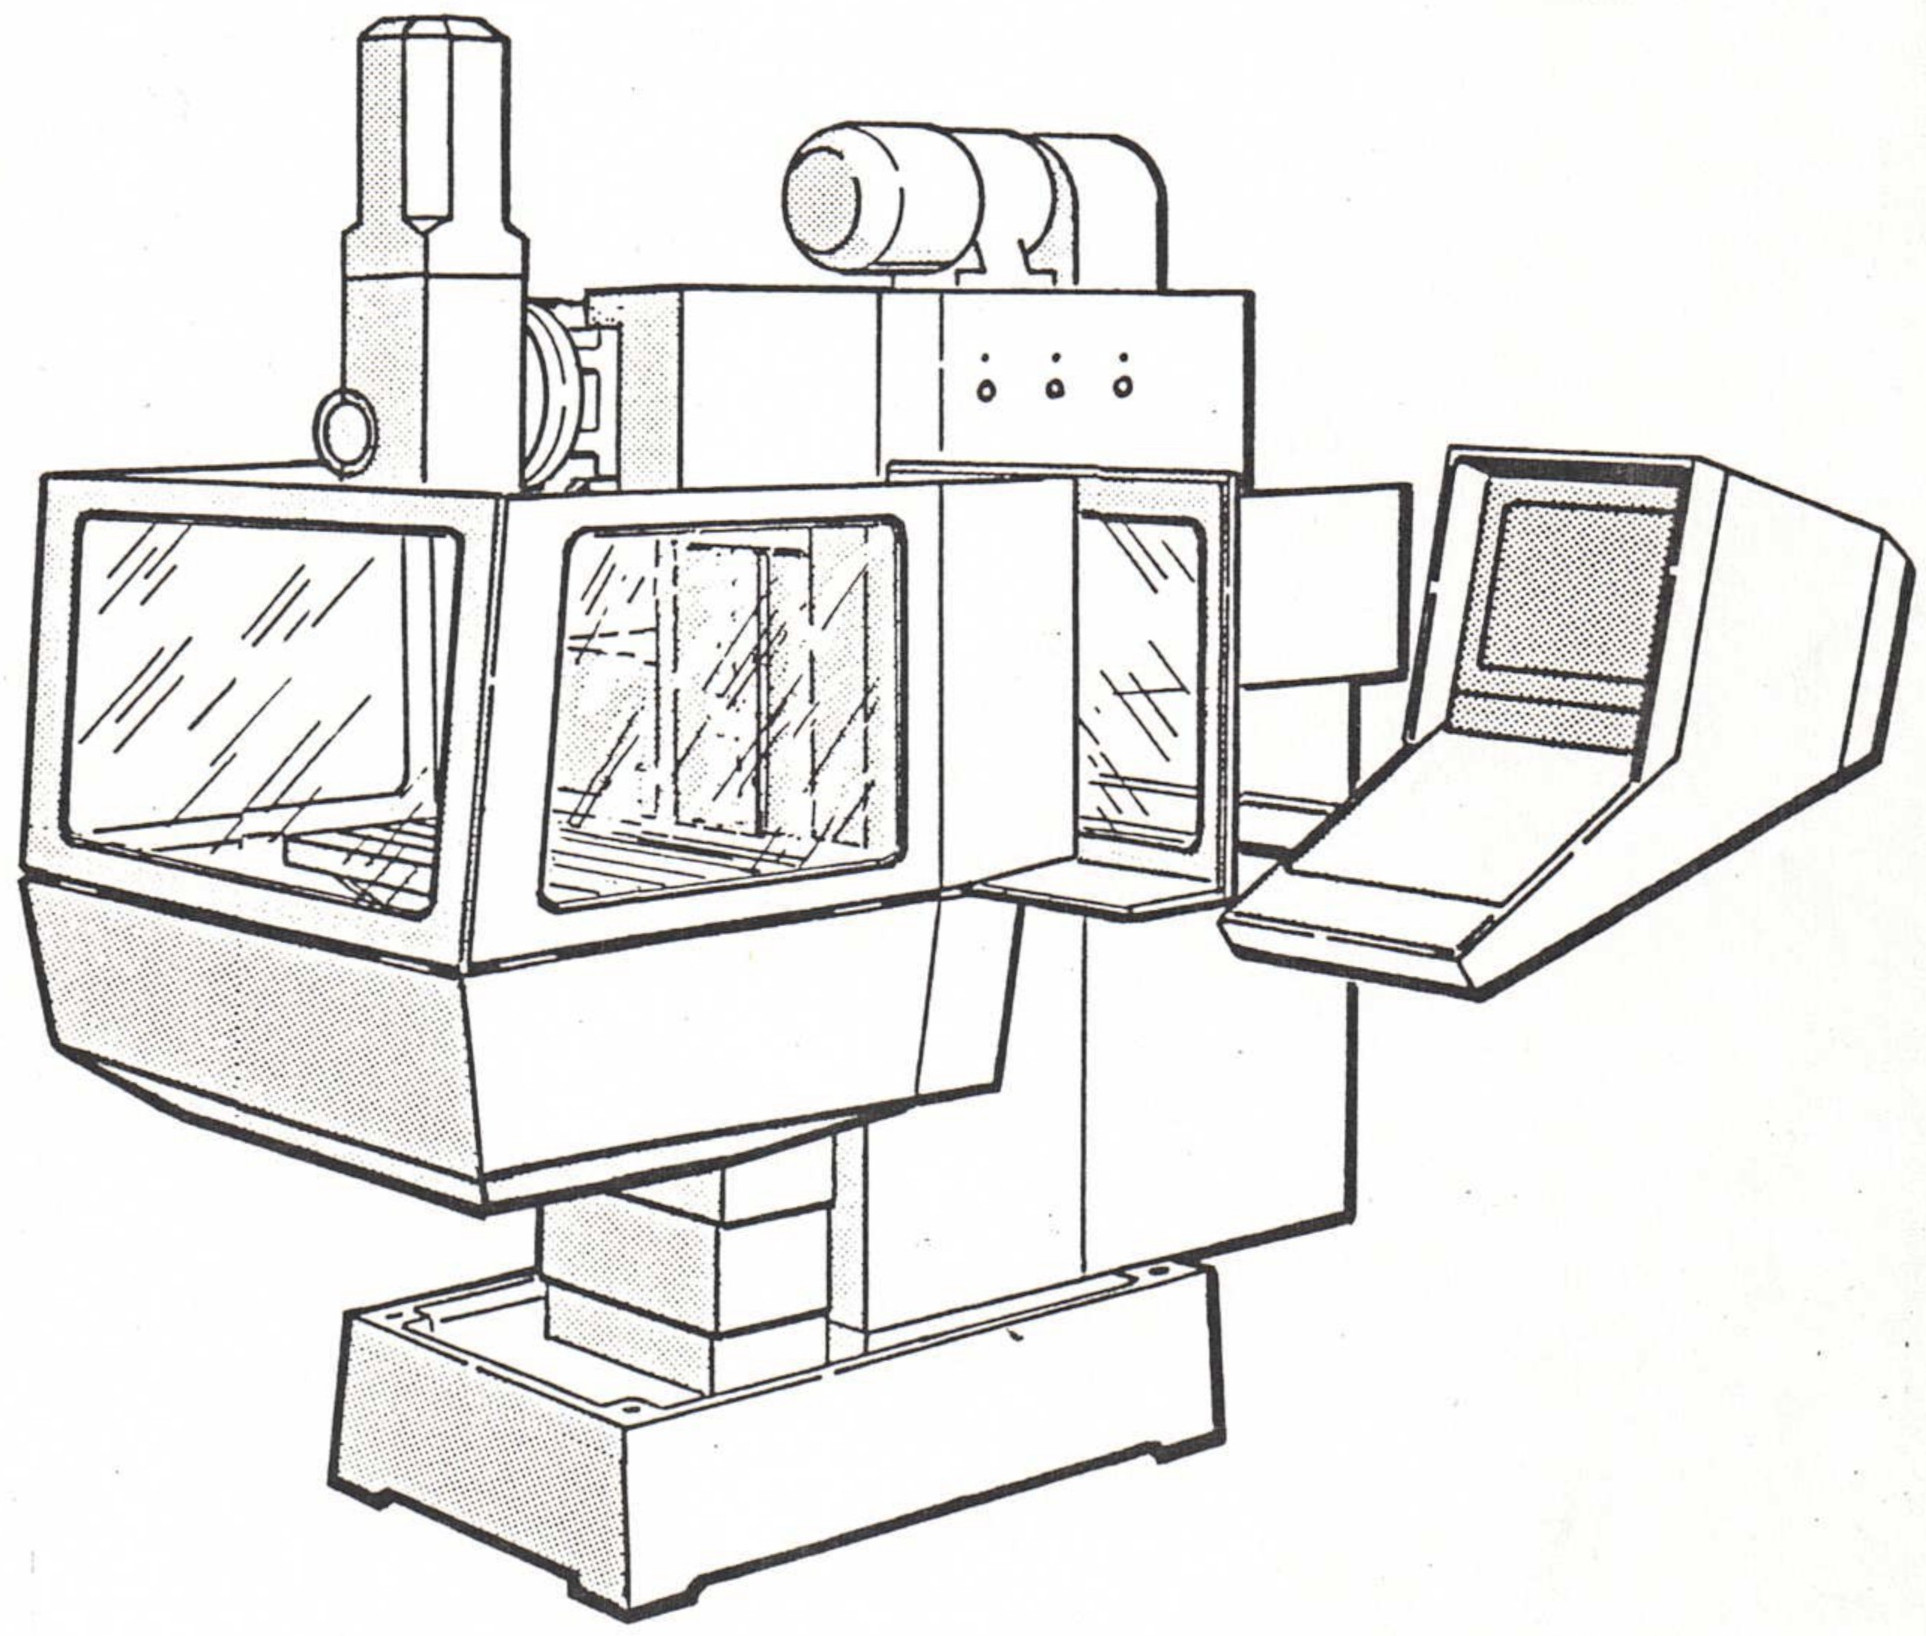
\includegraphics[width=0.9\textwidth]{chapter0/cover-image.jpg} 

        \vfill

         \noindent
         \begin{center}
             \parbox{\textwidth}{\centering {\Huge \textbf{Operation - Maintenance - Repair}}}
         \end{center}
    }
\end{titlepage}

\clearpage % Move to the next page and resume normal styling
\pagestyle{fancy} % Re-enable the default layout

\setsectiontitle{To our customers}
\setcounter{chapter}{0}
\setcounter{section}{0}

This operator's manual contains the essential information required for the proper operation and maintenance of your MAHO machine tool. It belongs in the hands of the operating and maintenance personnel.

The present operator's manual includes the separate operating instructions for CNC 432/10 graphics, the programming instructions for CNC 432 of the control unit, the programming manual for the \enquote{Geometry Package}, and the folder \enquote{Assembly Drawings and Parts Lists}.

Tax-specific details are listed \textbf{only} in the operating manual for CNC 432/10 graphics and should be referenced there.

The machine may only be put into operation after the operating and maintenance personnel have carefully read the operator's manual and have thoroughly\\ familiarized themselves with all details.

Operation and maintenance of the machine must be carried out in accordance with the instructions provided in this operator's manual.

\notebox{NOTE}{\textbf{We assume no liability for damages resulting from failure to follow these instructions or from improper handling.}}

If malfunctions occur that cannot be resolved independently, the cause of the malfunction should be determined using the operator's manual before \\contacting the appropriate MAHO representative or the MAHO company.

This operator's manual is designed to help you complete your machining tasks efficiently. We are confident that the delivered MAHO machine tool will fully meet your expectations. \\[1cm]

\noindent
\textbf{\textcopyright\ Copyright} \\[0.2cm]

This technical manual may \textbf{not}, even in part, be reproduced or made accessible to third parties without the express permission of the publisher.

\newpage

\subsection{Page Numbering}

The pages of this manual are numbered sequentially within each chapter \\according to sections. The page numbers are displayed in the upper right corner and are structured so that the page number follows the section number.

\textbf{EXAMPLE}: \texttt{3.20-3}, means Chapter 3, Section 20, Page 3.

If expansions occur within a section, these are numbered using the page number of the previous page followed by the numbers 1, 2, 3, etc., separated by a period.

\textbf{EXAMPLE}: \texttt{3.20-3.1}, means Chapter 3, Section 20, Page 3, Supplementary Page 1.

Figures and tables are not separately numbered.

The position numbers in the figures refer to the content of the section and can span 2-3 figures.

If positions of a figure are referenced in the text, they are placed within parentheses \texttt{()}.

\subsection{Notices in this Manual}

The following notices are used in this manual:

\notebox{NOTICE}{Applies to technical details that the user must observe.}

\notebox{CAUTION}{Applies to work or operational procedures that must be followed precisely to prevent damage or destruction of the system.}

\notebox{WARNING}{Applies to work or operational procedures that must be followed precisely to prevent hazards to personnel. This also includes \textbf{CAUTION}.}

\subsection{Cross-References}

To avoid redundant descriptions, content-related connections are established in this manual using cross-references.

\textbf{EXAMPLE}:
\begin{quote}
\noindent \hspace{-0.25cm} .... according to instructions .... \\
\hspace{1.3cm} .... see Sheet/Page ....
\end{quote}

\subsection{Location Definition}

The designations front, back, left, right, top, and bottom are based on the perspective from the spindle head looking toward the workpiece.

\setsectiontitle{Table of Contents}
\renewcommand{\arraystretch}{1.3} % Adjust row spacing for readability

\begin{tabularx}{\textwidth}{X r}
    \textbf{\underline{Commissioning the Machine}} & \\ % Main Section (No page number)
    Important Notes \dotfill & 1.01-1 \\
    Transport of the Machine \dotfill & 1.02-1 \\
     & 1.02-2 \\ % No extra &
    Setting Up the Machine \dotfill & 1.03-1 \\
     & 1.03-2 \\
     & 1.03-3 \\
    Setup Plan and Workspace Layout \dotfill & 1.04-1 \\
    Dimensional Drawing of the Machine \dotfill & 1.05-1 \\
    Removal of Rust Protection Agent \dotfill & 1.08-1 \\
    Spindle head oil fill \dotfill & 1.09-1 \\
    Connecting to the Electrical Network \dotfill & 1.10-1 \\
    Commissioning Checklist \dotfill & 1.11-1 \\[0.5cm]

    \textbf{\underline{General Description of the Machine}} & \\ % Main Section
    Technical Data \dotfill & 2.01-1 \\
     & 2.01-2 \\
    Machine Overview \dotfill & 2.02-1 \\
    Component Identification \dotfill & 2.02-2 \\
     & 2.02-3 \\
     & 2.02-4 \\
     & 2.02-5 \\
     & 2.02-6 \\
     & 2.02-7 \\
     & 2.02-8 \\
    Motion Directions \dotfill & 2.03-1 \\
    Control Station \dotfill & 2.04-1 \\
     & 2.04-2 \\
    Hand Control Panel \dotfill & 2.04-5 \\
    Gear Train Schematic \dotfill & 2.10-1 \\
    Main Gearbox \dotfill & 2.10-2 \\[0.5cm]

    \textbf{\underline{Machine Operation}} & \\
    Functional Testing - Trial Run \dotfill & 3.01-1 \\
     & 3.01-2 \\[0.5cm]
\end{tabularx}

\newpage

\begin{tabularx}{\textwidth}{X r}
    Manual Spindle Speed Selection \dotfill & 3.03-2 \\
    Horizontal Working Spindle \dotfill & 3.04-1 \\
    Horizontal Milling with Counter Holder \dotfill & 3.05-1 \\
    Horizontal to Vertical Conversion \dotfill & 3.07-1 \\
    Vertical to Horizontal Conversion \dotfill & 3.08-1 \\
    Vertical Milling Head without Quill Feed \dotfill & 3.09-1 \\
    Automatic Tool Clamping \dotfill & 3.12-1 \\
    Reworking of Standard Tool Shafts \dotfill & 3.13-1 \\
    Tool Shaft According to DIN 69871 \dotfill & 3.13-3 \\
    Manual Adjustment of the Machine Slide \dotfill & 3.15-2 \\
    Hydraulic Plan and Equipment List \dotfill & 3.18-1 \\
    Hydraulic System \dotfill & 3.18-3 \\
    Automatic Central Lubrication System \dotfill & 3.20-1 \\
    Equipment List - Automatic Central Lubrication \dotfill & 3.20-2 \\
    Automatic Central Lubrication \dotfill & 3.20-3 \\
     & 3.20-4 \\
     & 3.20-5 \\
    Coolant System \dotfill & 3.22-1 \\
    Splash Protection \dotfill & 3.24-1 \\[0.5cm]

    \textbf{\underline{Worktables}} & \\
    Fixed Angle Table \dotfill & 4.01-1 \\
     & 4.01-2 \\
    Universal Rotary Table \dotfill & 4.03-1 \\
     & 4.03-2 \\
     & 4.03-3 \\
     & 4.03-4 \\
     & 4.03-5 \\
     Angle Adjustment Display for B-Axis \dotfill & 4.04-1 \\[0.5cm]
\end{tabularx}

\newpage

\begin{tabularx}{\textwidth}{X r}
    \textbf{\underline{CNC Control}} & \\ % Main Section (No page number)
    Linear Measurement Systems and Display Units \dotfill & 5.01-1 \\
    Machine Constants CNC 432 \dotfill & E3.21741C \\
     & E3.21742C \\
     & E3.21743C \\
     & E3.21744C \\
     & E3.24628C \\
     & E3.24629C \\
     & E3.24630C \\
    Error List CNC 432 \dotfill & E3.22870C \\
     & E3.22871C \\
     & E3.22872C \\
     & E3.25024C \\
    Operating Manual CNC 432/Graphics \dotfill & 76.00471 \\
    Geometry Package for CNC 432/Graphics \dotfill & 76.00461 \\
    Programming Manual CNC 432 \dotfill & 76.00211 \\[0.5cm]

    \textbf{\underline{Accessories}} & \\ % Main Section
    High-Speed Milling Spindle \dotfill & 6.02-1 \\
    Dot-Matrix Printer ZIP 30 (Separate Manual) \\[0.5cm] % No page number

    \textbf{\underline{Maintenance}} & \\ % Main Section
    Important Notes \dotfill & 7.01-1 \\
    Machine Lubrication Plan \dotfill & 7.02-1 \\
    Lubrication Schedule \dotfill & 7.03-1 \\
    Lubricant Recommendations \dotfill & 7.06-1 \\
     & 7.06-2 \\
    Coolants \dotfill & 7.07-1 \\
     & 7.07-2 \\
     & 7.07-3 \\
     & 7.07-4 \\[0.5cm]
\end{tabularx}

\newpage

\begin{tabularx}{\textwidth}{X r}
    Removing the Machine Covers \dotfill & 7.10-1 \\
    Maintenance Plan \dotfill & 7.20-1 \\
    Overview of Maintenance Tasks for Mechanics and Hydraulics \dotfill & 7.21-1 \\
    Overview of Maintenance Tasks for Electrical and Electronics \dotfill & 7.22-1 \\
    Special Tools for Maintenance and Servicing \dotfill & 7.23-1 \\
    Adjusting the Gibs \dotfill & 7.30-1 \\
    Guideway Wiper Maintenance \dotfill & 7.31-1 \\
    Replacing the Feed Drive Timing Belt \dotfill & 7.33-1 \\
     & 7.33-2 \\
     & 7.33-3 \\
     & 7.33-5 \\
    Installation and Maintenance of the Poly-V Belt \dotfill & 7.34-1 \\
     & 7.34-2 \\
    Adjusting the Collet for Automatic Tool Clamping \dotfill & 7.35-1 \\
     & 7.35-2 \\
    Readjustment Work on the Universal Rotary Table \dotfill & 7.40-1 \\
     & 7.40-2 \\
    Maintenance of DC Motors \dotfill & 7.60-1 \\
     & 7.60-2 \\
     & 7.60-3 \\
    Maintenance of Three-Phase Motors \dotfill & 7.61-1 \\[0.5cm]

    \textbf{\underline{Spare Parts Plans and Lists}} & \\ % Main Section
    Notes on Ordering Spare Parts \dotfill & 8.00-1 \\
    Spare and Wear Parts List \dotfill & 99.34504 \\[0.5cm]

    \textbf{\underline{Disassembly Instructions}} & \\ % Main Section
    Main Motor \dotfill & 9.01-1 \\
    Replacing the Feed Motor \dotfill & 9.08-1 \\
     & 9.08-2 \\
     & 9.08-3 \\
\end{tabularx}

\notebox{NOTE}{The mandatory machine constants for the machine are supplied as punched tape and plaintext. They are located with the electrical circuit diagrams in the control cabinet of the machine.}

\refstepcounter{chapter}
\addcontentsline{toc}{chapter}{Before Starting the Machine}

\section{Important Notes}

\subsection{Factory Number}
\begin{itemize}
    \item The information in this operator's manual applies \uline{\textbf{only}} to the machine whose factory number is stamped on the machine's nameplate.
    \item For all inquiries and spare part orders, the factory number of the machine must be specified.
    \item If inquiries pertain to a specific page of the operator's manual, the page number must also be provided.
\end{itemize}

\subsection{Before Starting the Machine}
\begin{itemize}
    \item Carefully read the operator's manual.
    \item Set up the machine (see Page 1.03-1).
    \item Ensure that the machine has reached room temperature.
    \item Remove rust protection (see Page 1.08-1).
    \item Tighten all terminal screws on the terminal strips, contactors, relays, and fuses in the control cabinet; they may have loosened due to vibrations during transport.
    \item Connect the machine to the electrical network (see Page 1.10-1).
    \item Check oil levels (see Page 7.02-1 and 7.03-1).
    \item Fill the machine with coolant (see Page 3.22-1).
\end{itemize}

\subsection{Interlocks of the Machine}
\begin{itemize}
    \item After switching off the main switch -Q1- in the control cabinet and after every power failure, the machine must be restarted.\footnotemark[1]
    \item The red mushroom button of the EMERGENCY STOP switch must not be pressed during this process.
    \item After each EMERGENCY STOP, the corresponding mushroom button must be \\released by turning it clockwise, and the machine must be restarted.\textsuperscript{\footnotemark[1]}
\end{itemize}

\footnotetext[1]{"Start the machine", see separate CNC 432 operating instructions.}

\section{Transport of the Machine}

The dimensions and weights of the machine with the fixed table and coolant container are as follows:

\begin{table}[h]
\centering
\begin{tabular}{lll}
\textbf{Packaging Type} & \makecell{\textbf{Dimensions}\\\textbf{(L x W x H) [m]}} & \textbf{Weight [kg]} \\ \hline
EURO Packaging (Pallet/Carton) & $1.9 \times 1.8 \times 2$ & 1450 \\
Box (USSR) & $1.9 \times 1.9 \times 2.05$ & 1590 \\
Box (Seaworthy) & $2.35 \times 1.9 \times 2.05$ & 1693 \\
Container Loading (Machine on Pallet) & $1.8 \times 1.8 \times 1.98$ & 1362 \\
\end{tabular}
\end{table}

\begin{figure}[h]
    \centering
    \begin{minipage}[b]{0.35\textwidth} % Align to the bottom with [b]
        \centering
        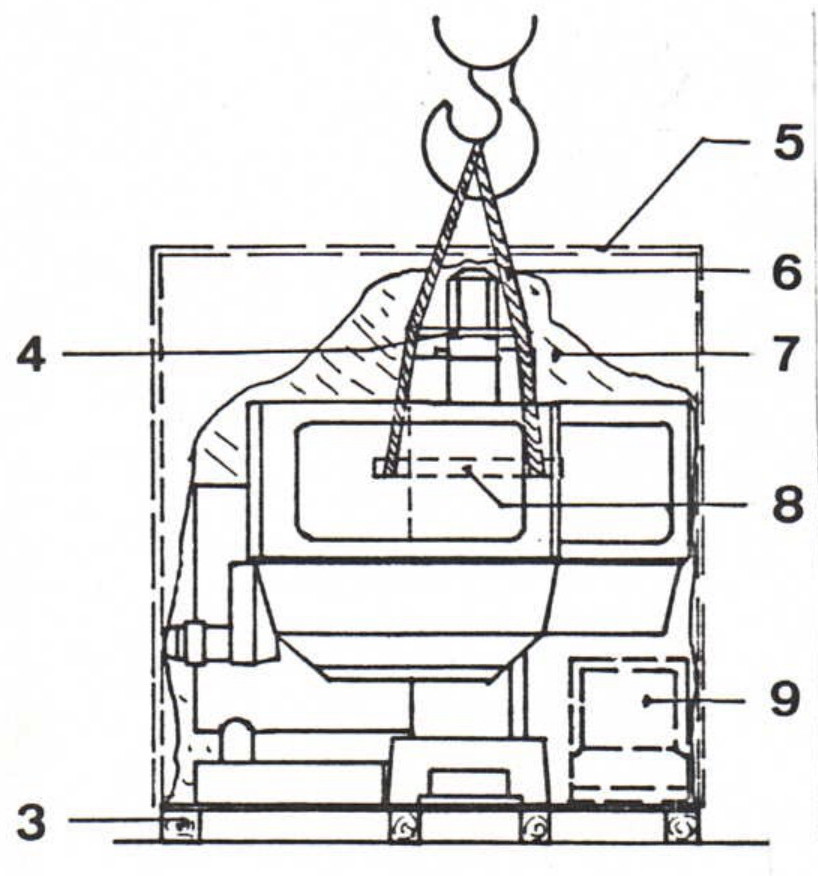
\includegraphics[width=\textwidth]{chapter1/machine_packaging_transport.jpg} % Replace with actual image file
        \caption{}
        \label{fig:packaging}
    \end{minipage}
    \hfill
    \begin{minipage}[b]{0.55\textwidth} % Align to the bottom with [b]
        \centering
        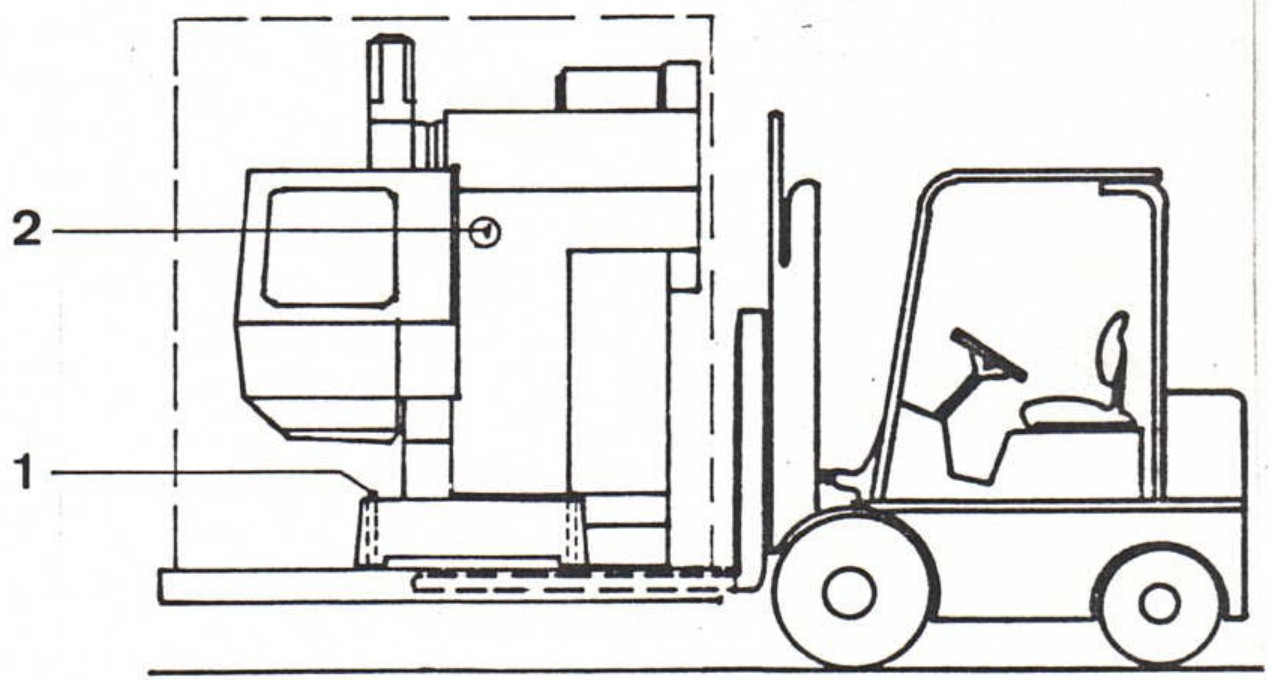
\includegraphics[width=\textwidth]{chapter1/machine_unloading_forklift.jpg} % Replace with actual image file
        \caption{}
        \label{fig:unloading}
    \end{minipage}
\end{figure}

\begin{itemize}
    \item Unload the packaged machine from the transport device using a forklift, hoist, or similar equipment.
    \item Remove the packaging (\textbf{5}) and cut and remove the protective foil (\textbf{7}) from the base of the box. Take off the sealing covers (\textbf{2}) on both sides.
    \item Check the machine and accessories for any transport damage.
\end{itemize}

\notebox{NOTE}{Damages or other defects, such as incompleteness, must be reported immediately in writing to the shipping company or railway, the insurance company, and the company MAHO.} 

\begin{itemize}
    \item Insert the transport rod (\textbf{8}) (maximum 50 mm diameter, 1000 mm length) into the opening in the stand.
    \item Attach the endless sling (\textbf{6}), with a minimum load capacity of 3000 kg and a total length of approximately 6 m, to the crane hook and the transport rod.
\end{itemize}

\notebox{CAUTION}{Place the detached control panel (\textbf{9}) on the work table and secure it against slipping!}

\sectionLikeSubsection{Transport of the Machine}

\begin{itemize}
    \item Perform a hanging test, i.e., align the machine by moving the transport rod (\textbf{8}) in the stand so that it hangs horizontally. Using a spacer (\textbf{4}) prevents the rope from rubbing against the machine.
    
    \item Lower the machine, unscrew the fastening nuts (\textbf{1}), and remove the pallet or box bottom (\textbf{3}) after lifting the machine again.
\end{itemize}

\textbf{When using a forklift:} Place the machine on wooden boards laid on the forks of the forklift (Fig. \ref{fig:unloading}) or hang it on the forks using a rope (Fig. \ref{fig:machine_placement_forklift}).
    
In unfavorable space conditions, use the "Transport Mule" (Fig. \ref{fig:machine_placement_mule}).

\begin{itemize}
    \item Transport the machine to the prepared location according to Page 1.03-1 and carefully place it on the damping plates provided.
\end{itemize}

\begin{figure}[h]
\centering
\begin{minipage}[t]{0.45\textwidth}
    \centering
    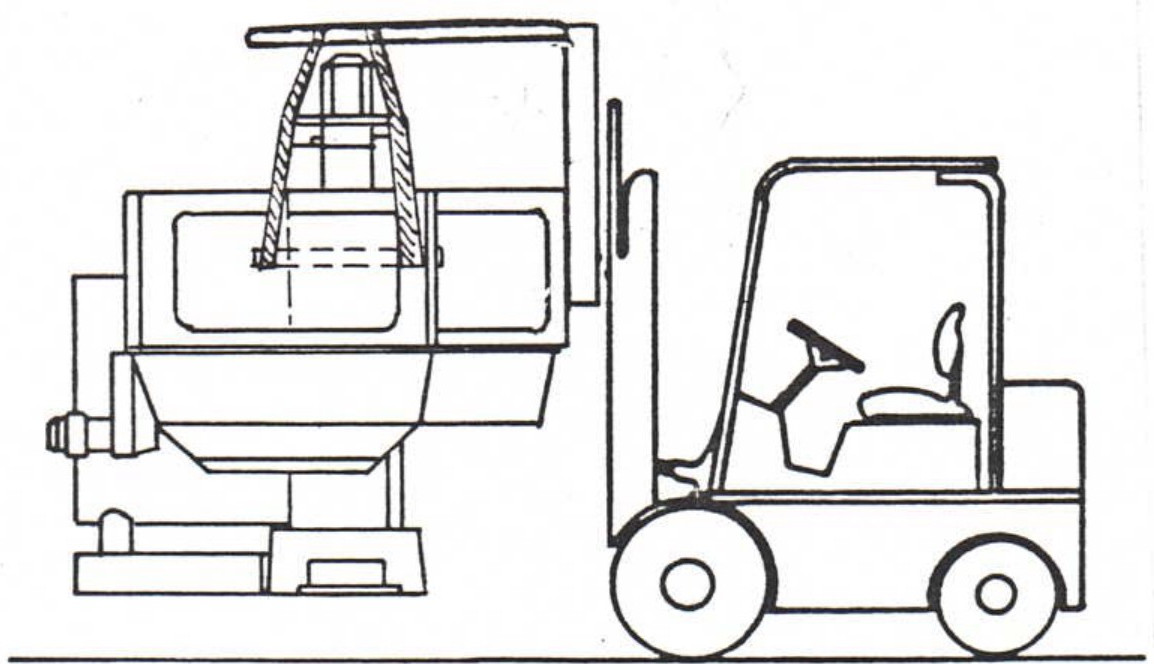
\includegraphics[width=\textwidth]{chapter1/machine_placement_forklift.jpg} % Replace with actual image file
    \caption{}
    \label{fig:machine_placement_forklift}
\end{minipage}
\hfill
\begin{minipage}[t]{0.45\textwidth}
    \centering
    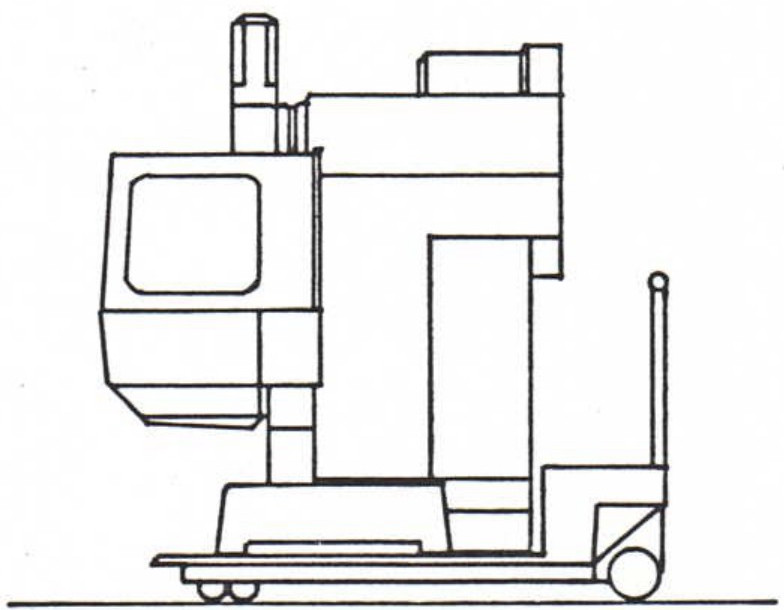
\includegraphics[width=\textwidth]{chapter1/machine_placement_mule.jpg} % Replace with actual image file
    \caption{}
    \label{fig:machine_placement_mule}
\end{minipage}
\end{figure}

\vspace{1em}

\infoBullet{Setup plan and workspace layout}{1.04-1}

\section{Installation of the Machine}

\subsection{Installation Site}
To ensure proper functionality of the machine, the following points regarding the installation site must be observed:
\begin{itemize}
    \item It must be free from vibrations.
    \item It must be free from local, one-sided heating or cooling of the machine, e.g., sunlight, radiators, drafts, etc.
    \item It must be free from interfering electrical installations (high-frequency).
    \item The total floor area requirement ($A_\text{WMP}$) is $3.2 \times 3.4 \, \text{m}$ ($10.88 \, \text{m}^2$).
    \item Within this total area, the machine covers an area of $3.5 \, \text{m}^2$, for which a minimum load-bearing capacity of $400 \, \text{daN/m}^2 \, (0.40 \, \text{t/m}^2)$ must be ensured.
    \item Ideally, the floor should be concrete or wood block.
\end{itemize}

\notebox{CAUTION}{
Mixed floors, i.e., machine standing on both concrete and wood block, are not permissible.
}

\begin{itemize}
    \item The unevenness of the floor must not exceed $3 \, \text{mm/m}^2$.
    \item A constant room temperature of max. $30^\circ \text{C}$ ($303 \, \text{K}$) must not be exceeded.
    \item The relative humidity must not exceed $80\%$.
\end{itemize}

\notebox{NOTE}{
Higher humidity or room temperatures up to $55^\circ \text{C}$ ($328 \, \text{K}$) are permissible when using MAHO cooling units in the command station and control cabinet.
}

\infoBullet{Setup plan and workspace layout}{1.04-1}\\
\infoBullet{Dimensions of the machine}{1.05-1}

\newpage
\sectionLikeSubsection{Setup of the Machine}

\begin{itemize}
    \item Lay out the supplied \enquote{Airlock damping plates} (1) according to the following sketch.
    \item Carefully place the machine on the damping plates.
    \item Leveling in the Z-direction (using shims) is necessary to ensure the oil level in the spindle head is maintained accurately!
    \item Position the coolant tank (2) accordingly, and screw the coolant pump (3) and return line (5) into the tank lid (4).
\end{itemize}

\vspace{1cm}

\begin{figure}[h!]
    \centering
    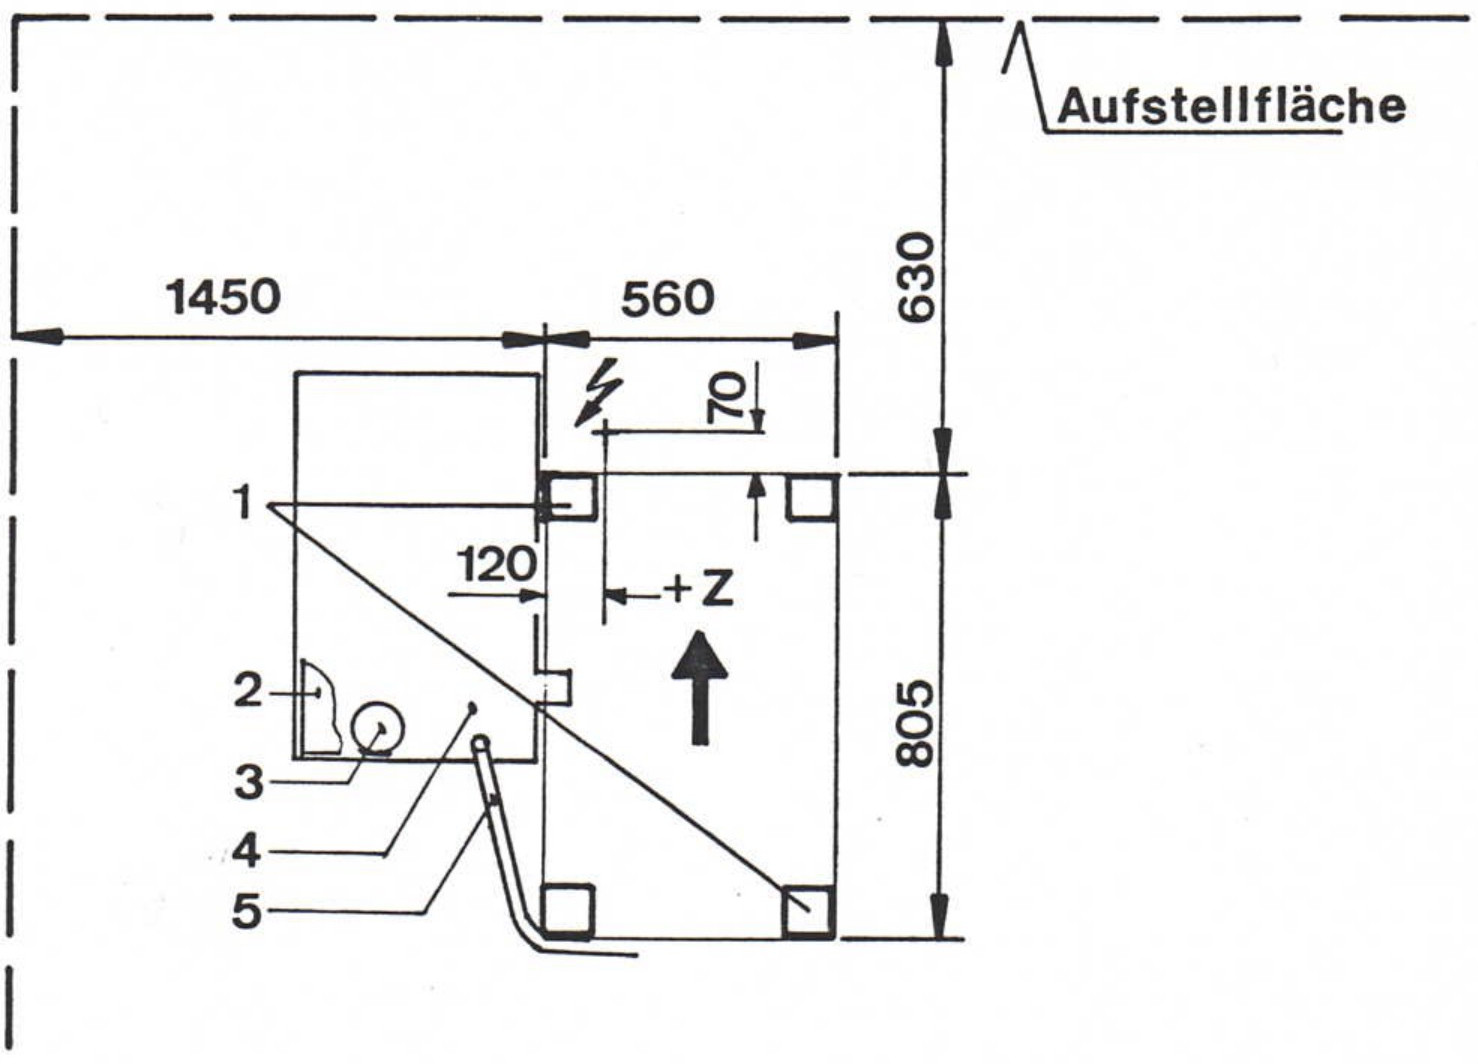
\includegraphics[width=\textwidth]{chapter1/machine_setup_sketch.jpg}
    \caption{Sketch for machine setup, including leveling and coolant system placement.}
    \label{fig:machine_setup_sketch}
\end{figure}

\sectionLikeSubsection{Mounting the Control Panel}

\begin{itemize}
    \item Remove the cover (7) and, if necessary, (9).
    \item Pull the pivot pin (8) out of the support (14).
    \item Place the extension arm (11) onto the support (14), slide the fork end \\(11.1) over the stop screw (12), and insert the cable bundle (13) into the bottom opening of the extension arm (11).
    \item Insert the pivot pin (8) into the extension arm (11) and the support (14). Tighten the mounting bracket of the cable hose (15) \\onto the extension arm.
    \item Insert the control panel (5) into the extension arm (11).
\end{itemize}

\begin{figure}[h!]
    \centering
    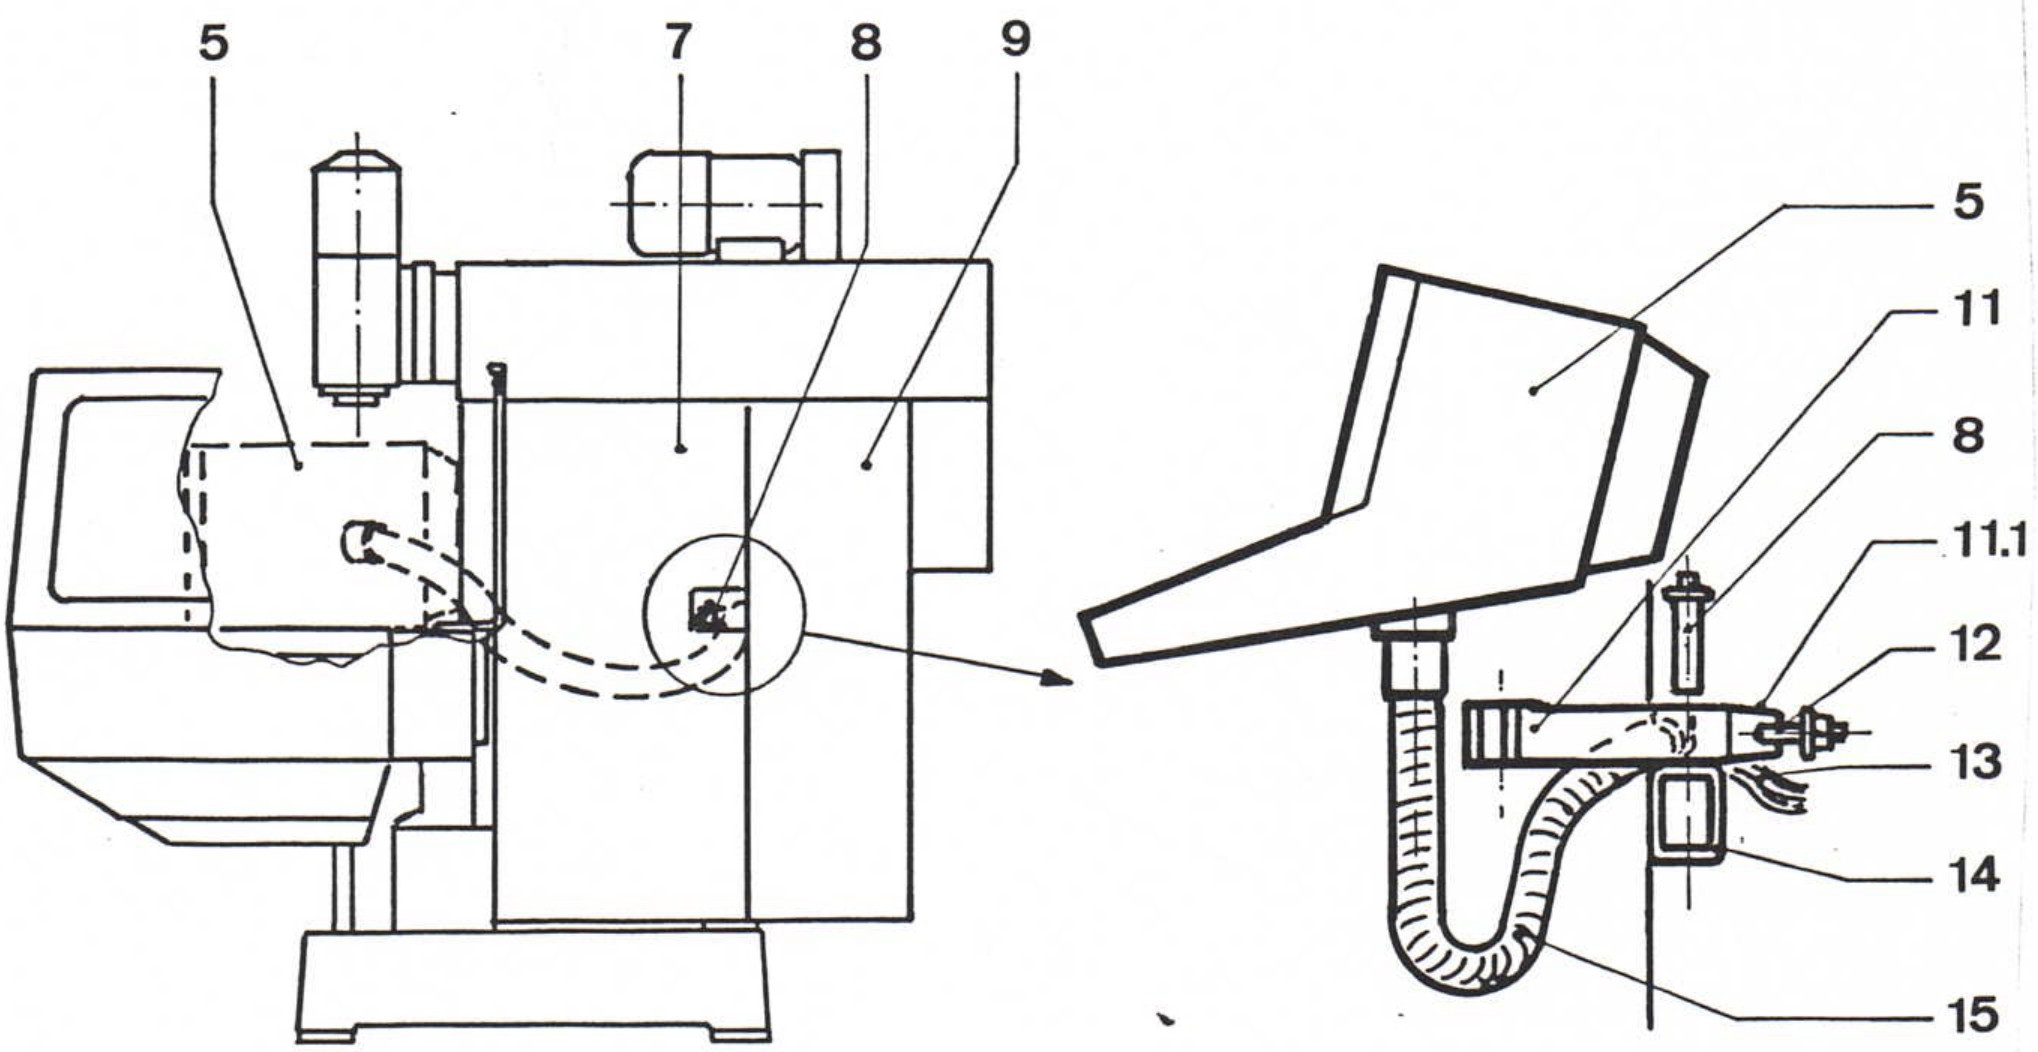
\includegraphics[width=\textwidth]{chapter1/control_panel_mounting_diagram.jpg}
    \caption{}
    \label{fig:control_panel_mounting}
\end{figure}

\section{Setup Plan and Workspace Layout}

\begin{description}[labelwidth=4cm, labelindent=0cm, leftmargin=0cm, rightmargin=2cm]
    \item[Total space requirement:] \dotfill 10.5 m\textsuperscript{2}
    \begin{itemize}
        \item Area for maintenance and disassembly \dotfill 5.06 m\textsuperscript{2}
        \item Machine footprint \dotfill 0.42 m\textsuperscript{2}
        \item Operator space \dotfill 3.8 m\textsuperscript{2}
        \item Setup area \dotfill 1.6 m\textsuperscript{2}
        \item Coverage area (F) \dotfill 3.25 m\textsuperscript{2}
    \end{itemize}
    \item[Height of the machine:] \dotfill 1.83 m
    \item[Weight of the machine (total):] \dotfill approx. 1,250 kg
    \item[Floor load on area (F):] \dotfill approx. 400 kg/m\textsuperscript{2}
\end{description}

\begin{figure}[H]
    \centering
    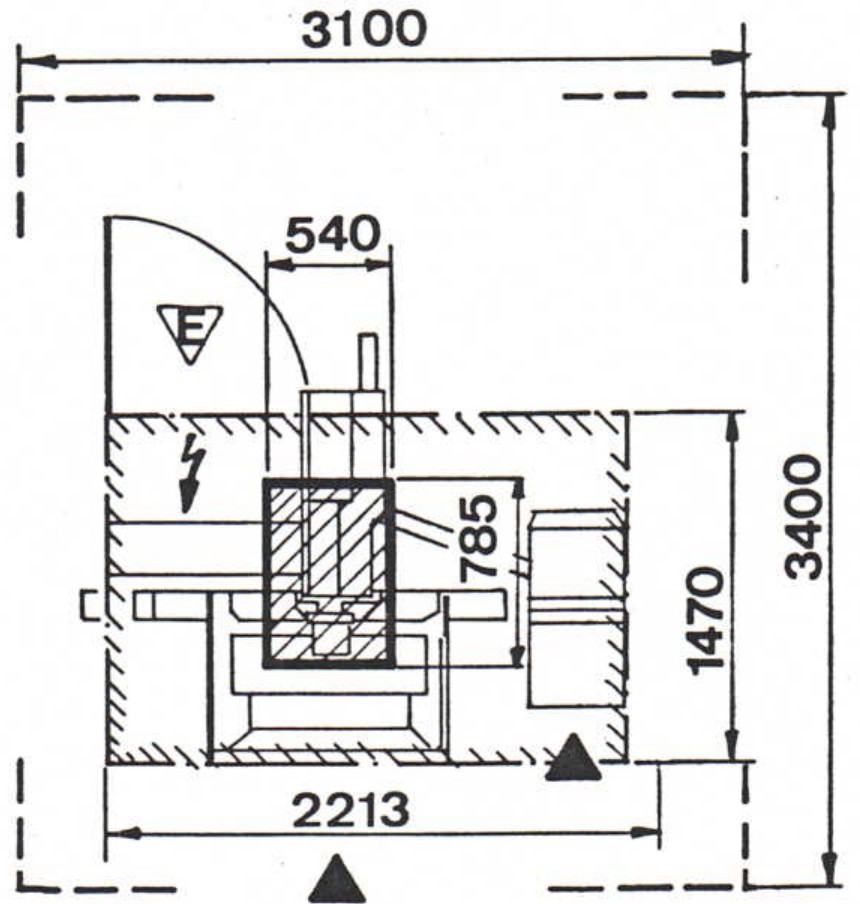
\includegraphics[width=0.45\textwidth]{chapter1/setup_plan_workspace_layout_diagram.jpg}
    \caption{}
    \label{fig:setup_plan_workspace_layout}
\end{figure}

\begin{description}[labelwidth=0cm, labelindent=0cm, leftmargin=0cm]
    \item \adjustbox{valign=c}{
\includegraphics[height=1cm]{chapter1/icon_electrician_access.jpg}} \hspace{0.5cm} Electrician access
    \item \adjustbox{valign=c}{
\includegraphics[height=1cm]{chapter1/icon_coverage_area.jpg}} \hspace{0.5cm} Coverage area (F)
    \item \adjustbox{valign=c}{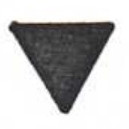
\includegraphics[height=1cm]{chapter1/icon_operator_position.jpg}} \hspace{0.5cm} Operator position
\end{description}

\vspace{-\topsep} % Suppress extra vertical space above the block
\begin{minipage}{\textwidth}
    \begin{minipage}[t]{1.5cm} % Adjust the width for the icon
        \raggedright
        \raisebox{-0.5\height}{% Adjust vertical alignment of the icon
            
\includegraphics[height=1cm]{chapter1/icon_electrical_connection.jpg}
        }
    \end{minipage}%
    \begin{minipage}[t]{\dimexpr\textwidth-1.5cm\relax} % Remaining space for text
        \begin{description}[labelwidth=6cm, labelindent=0cm, leftmargin=7cm, itemsep=0pt]
            \item[Power connection:] \dotfill 11 kVA
            \item[Free cable length across the floor:] \dotfill 0.5 m
            \item[Maximum fuse rating:] 
            \begin{itemize}[itemsep=0pt, topsep=0pt]
                \item 200-220 V \dotfill 35 A
                \item 380-500 V \dotfill 25 A
            \end{itemize}
        \end{description}
    \end{minipage}
\end{minipage}

\section{Dimensional Drawing of the Machine}

\begin{figure}[H]
    \centering
    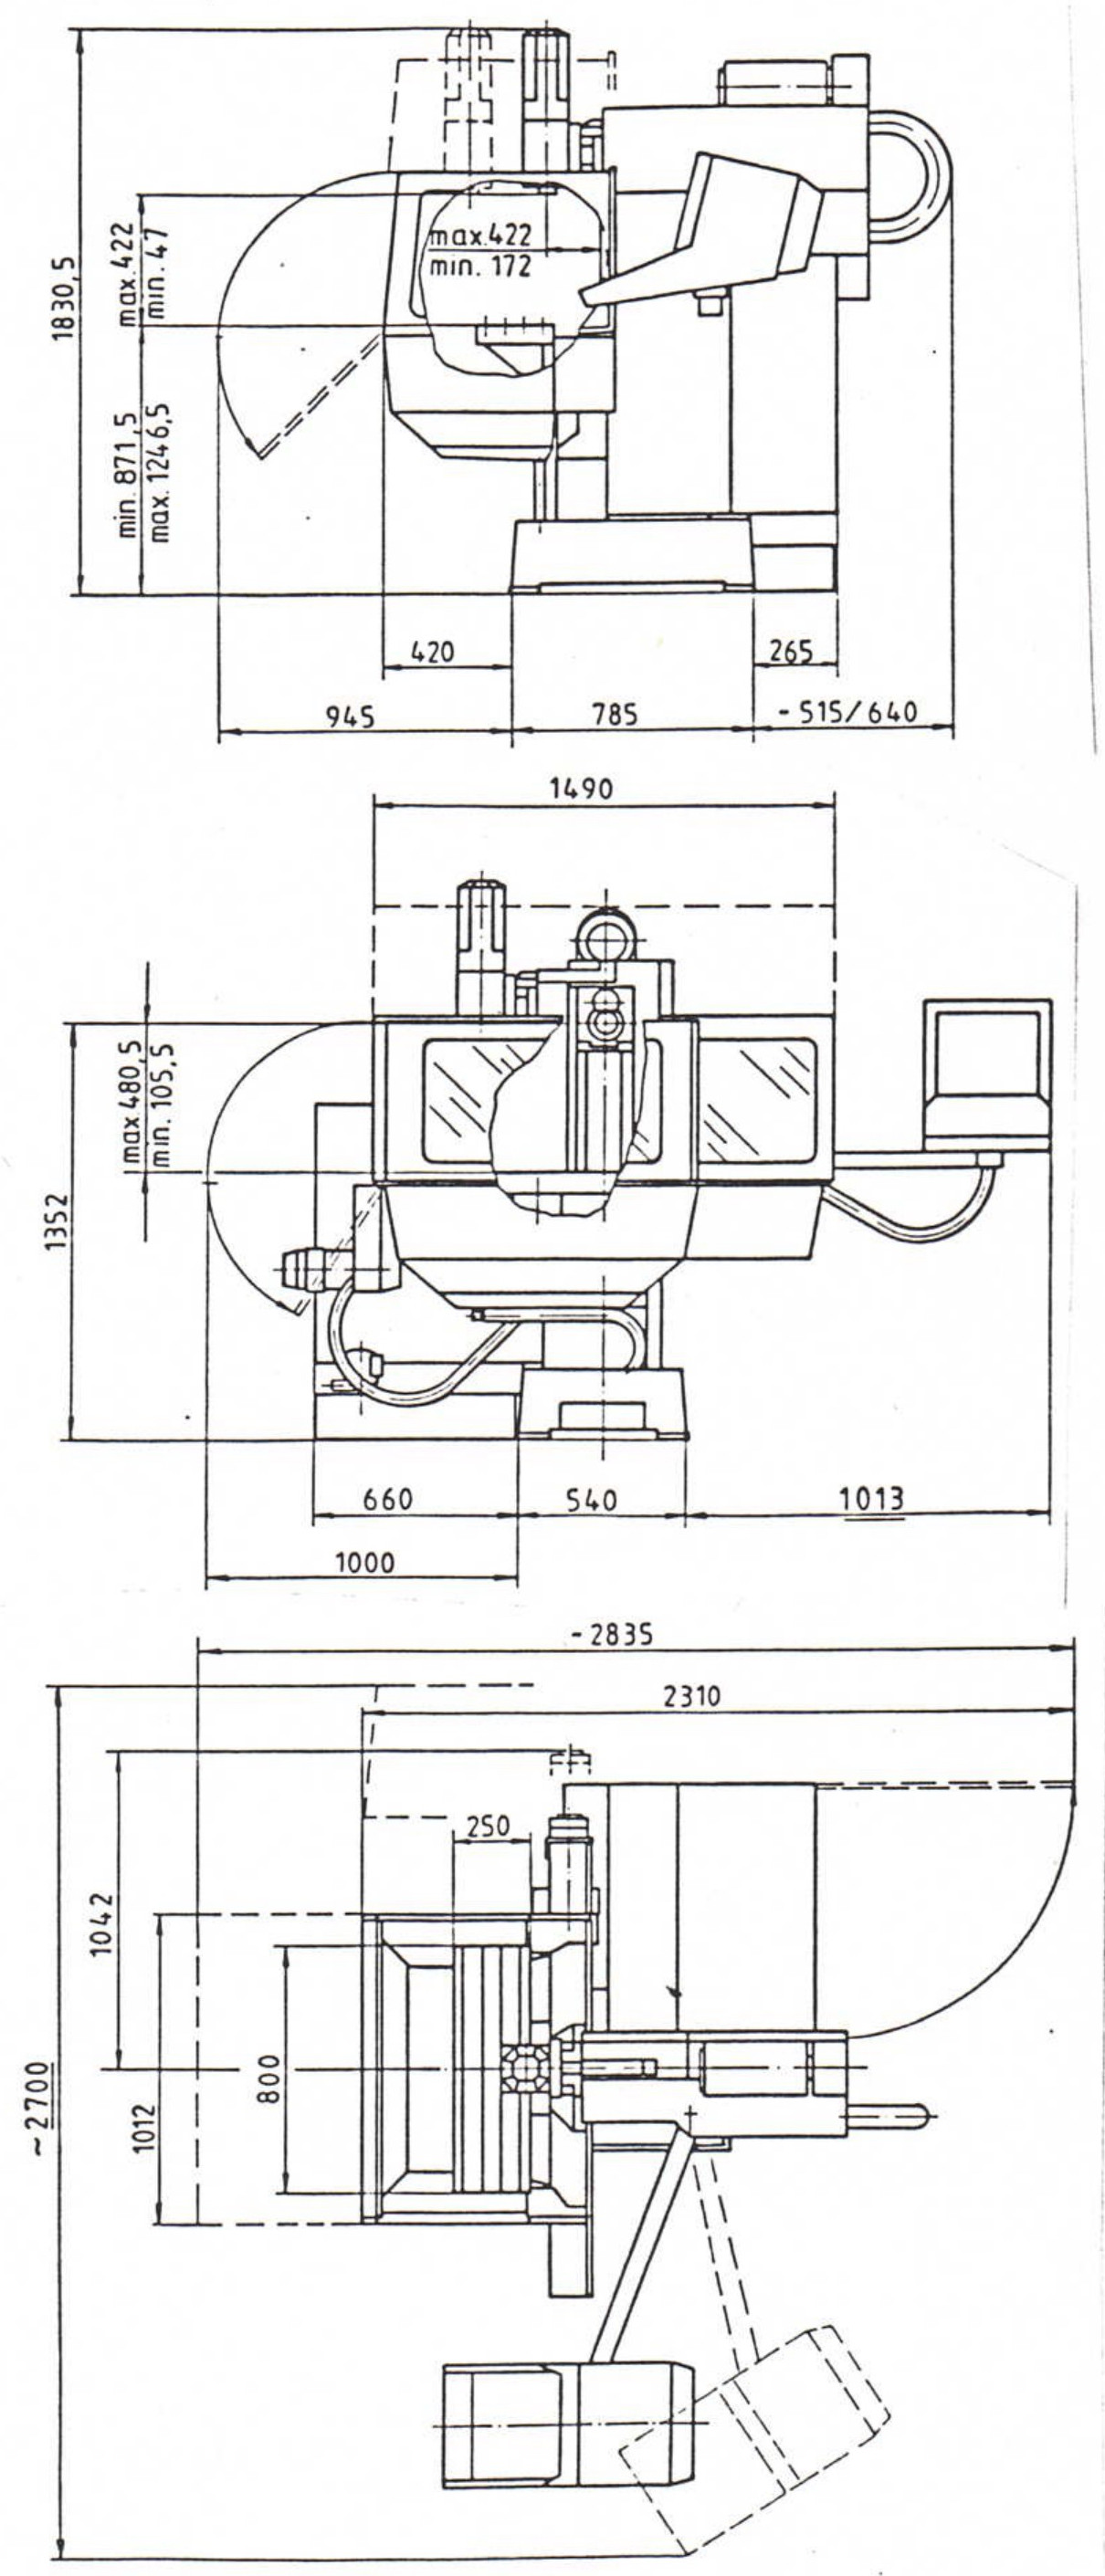
\includegraphics[width=.55\textwidth]{chapter1/machine_dimensions.jpg}
    \caption{}
    \label{fig:setup_plan_workspace_layout}
\end{figure}


\section{Removal of the Rust Protection Agent}

\setcounter{section}{8}

\notebox{WARNING}{Before removing the rust protection agent from the machine, no adjustments to the slides must be made.}

\begin{figure}[h]
    \centering
    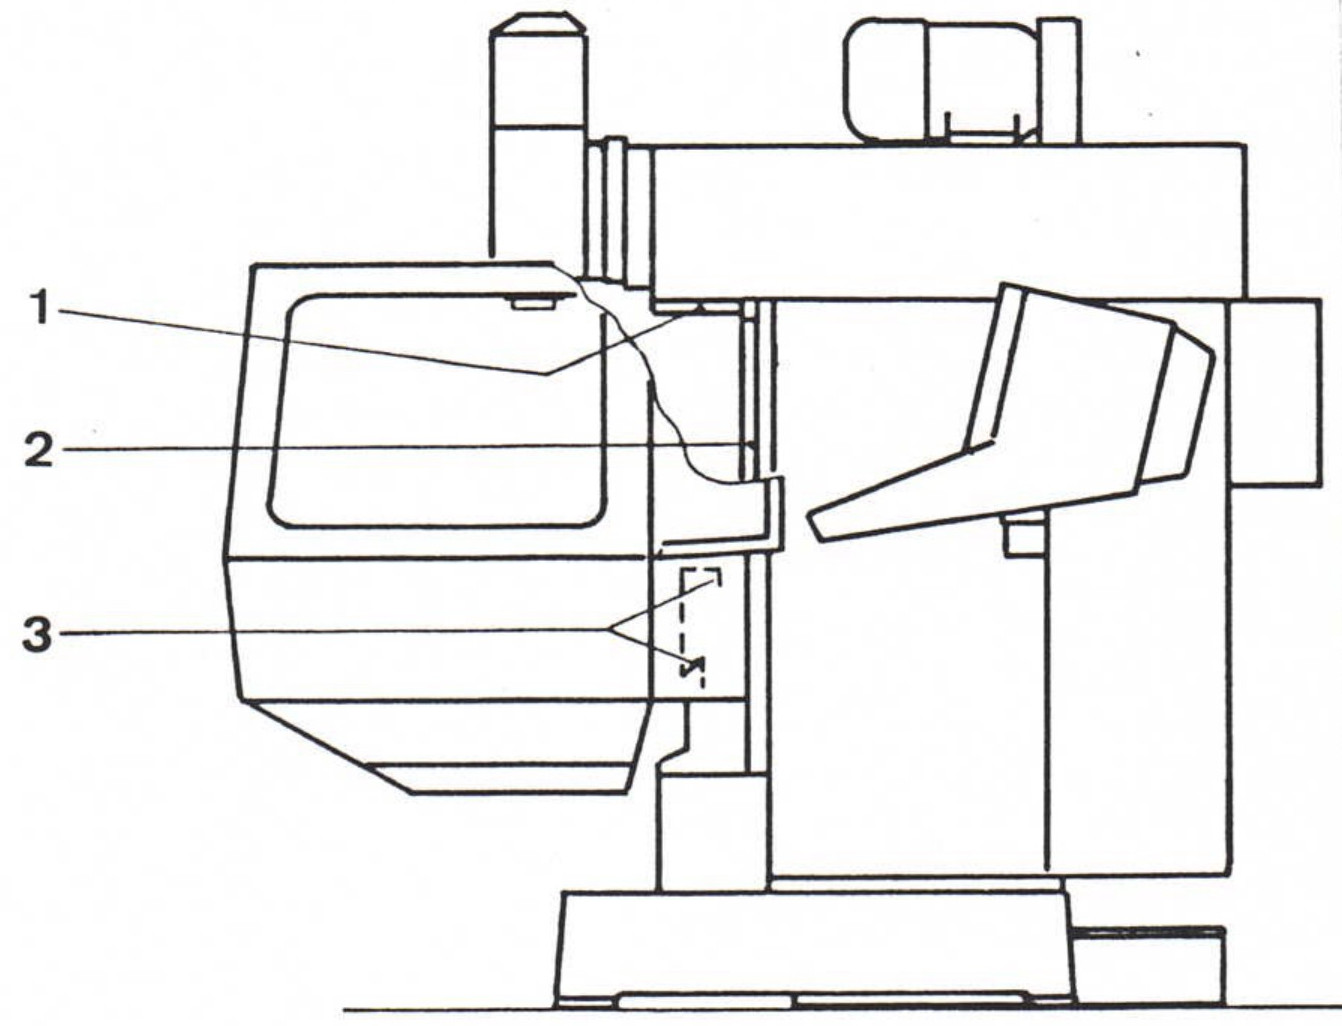
\includegraphics[width=0.7\textwidth]{chapter1/diagram_removal_of_rust_protection_agent.jpg}
    \caption{}
\end{figure}

\begin{itemize}
    \item Carefully remove the rust protection agent from the bare external surfaces and the receptacle cones of the work spindles using a soft cloth soaked with petroleum, gasoline, tetra, or another solvent for hydrocarbons.
    \item \textbf{Do not under any circumstances use scrapers or other sharp tools for this task.}
    \item Clean the sliding surfaces of the dovetail guides of the headstock (1) and the cross slide (2) with a soft cloth to remove the rust protection grease and apply oil with a brush.\footnotemark[2]
    \item Clean accessible sliding surfaces of the combined dovetail flat guides (3) of the vertical clamping table with a soft cloth to remove the rust\\ protection grease and apply oil.
\end{itemize}

\footnotetext[2]{The oil used in the central lubrication system must be applied (see page 7.06-1 \enquote{Lubricant Recommendations}).}

\notebox{WARNING}{Mixing of oils must be strictly avoided.}

\section{Filling the Drive Gear Oil Reservoir in the Spindle Head}

To prepare the machine for operation, the oil in the work spindle drive must be drained during transport and refilled before commissioning.

\vspace{.5cm}

\notebox{CAUTION}{Verify that the machine is level in the Z-axis using a spirit level, and adjust if necessary.\footnotemark[3]}

\footnotetext[3]{See Sheet 1.03-1.}

\begin{itemize}[itemsep=0.5em]
    \item Unscrew the front fill screw (1).
    \item Using the supplied container labeled "CLP 46/HLP 46" (Aral Sumorol CM 46), pour 0.2 liters into a measuring container and fill it into the fill opening (2) on the spindle head.
    \item Wait approximately 10 minutes, then read the oil level in the sight glass. If necessary, refill the remaining quantity in steps of 0.1 liters using the measuring container until the oil level reaches the corresponding mark (3).
    \item Reattach the fill screw (1).
\end{itemize}

\begin{figure}[h!]
    \centering
    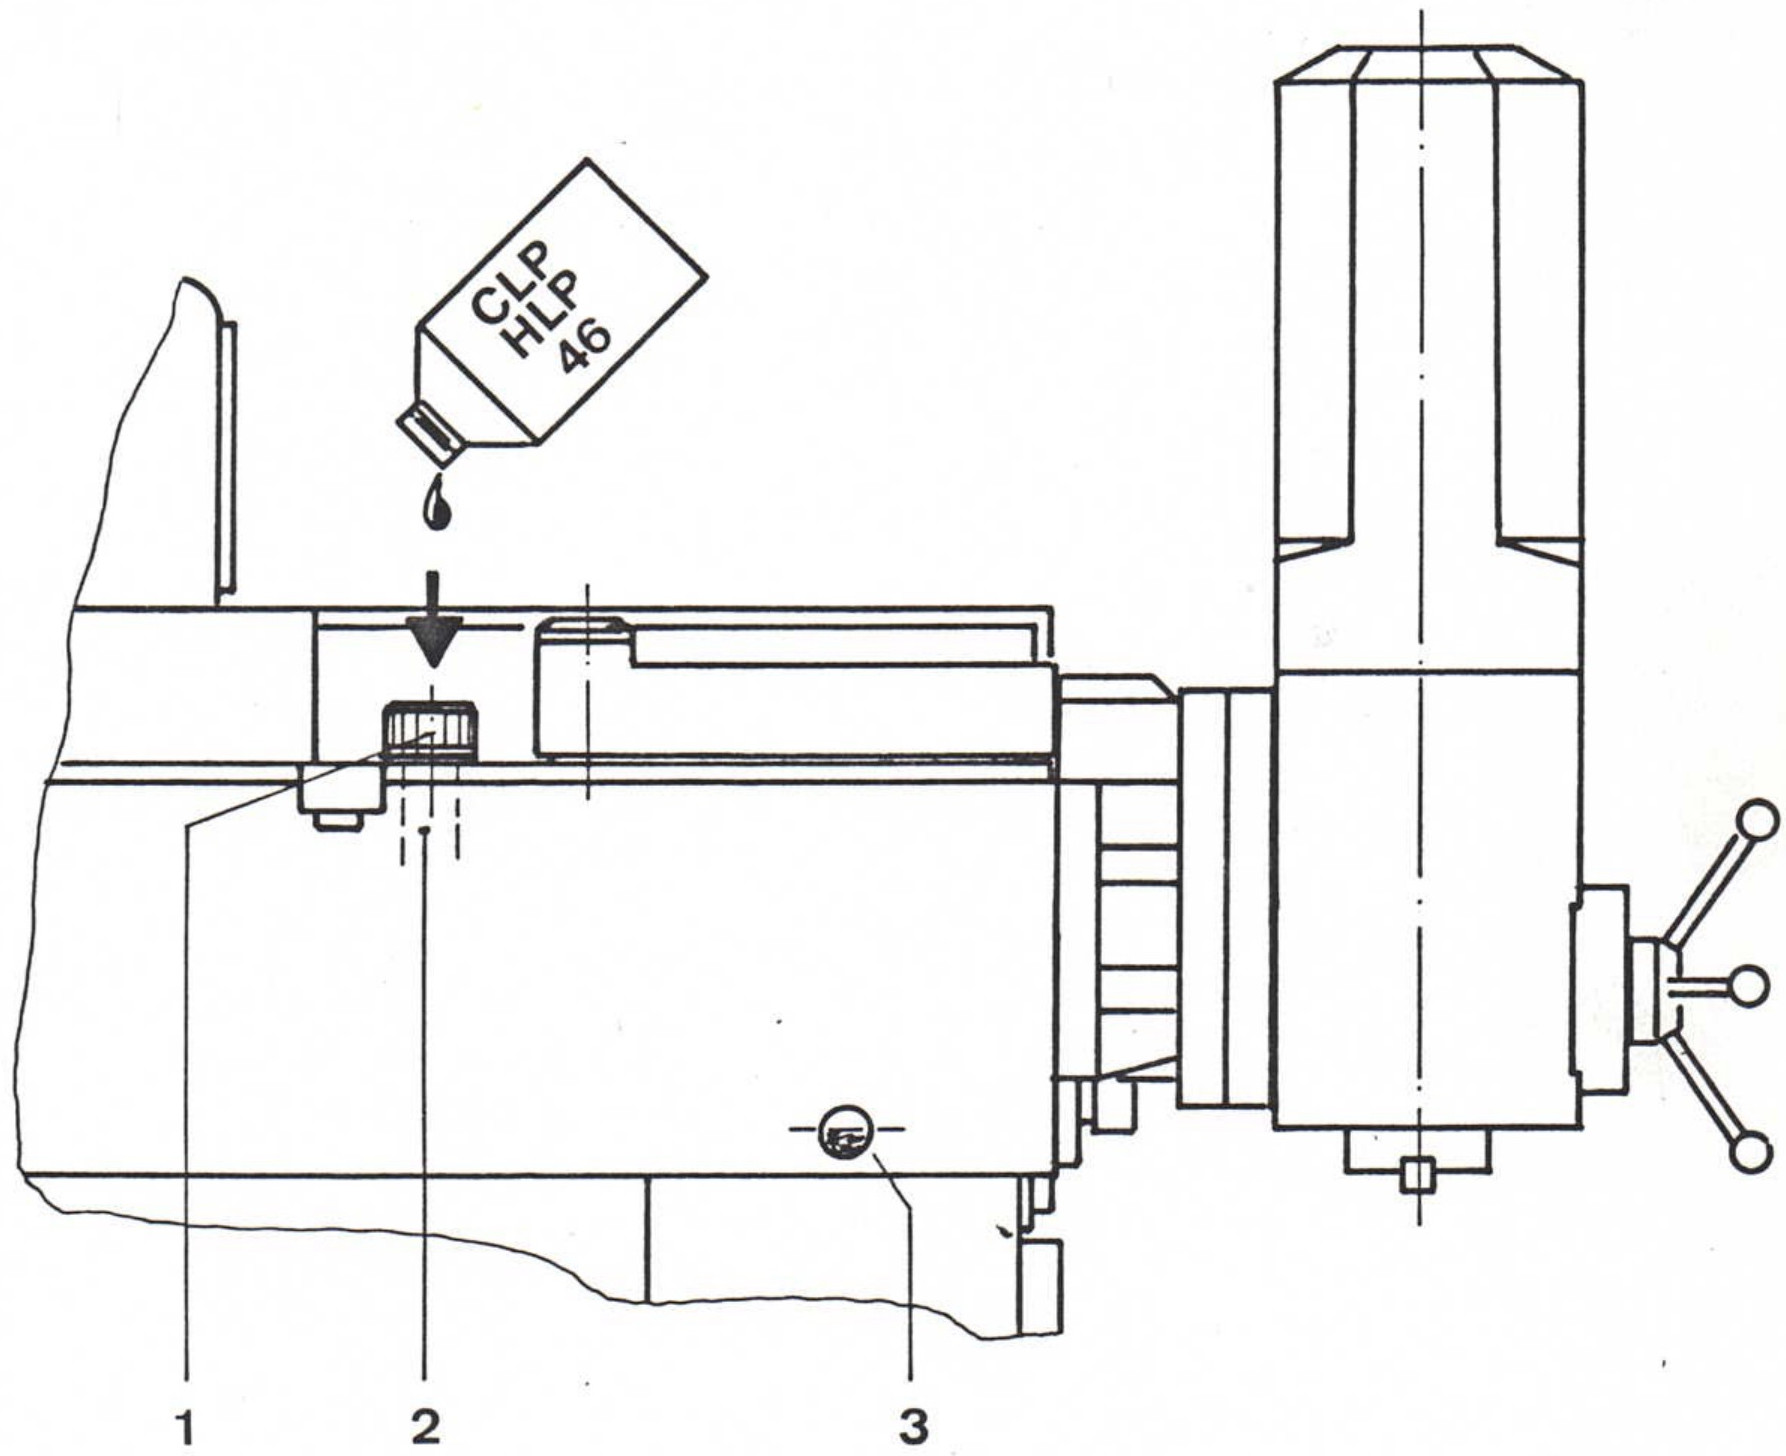
\includegraphics[width=0.8\textwidth]{chapter1/spindle_oil_fill_diagram.jpg} % Replace with your image filename
    \caption{}
\end{figure}


\section{Connecting to the Electrical Network}

Connection regulations from the responsible power supply company must be observed.

\begin{figure}[htp] % Top alignment for the figure
    \centering
    \begin{minipage}[t]{.4\linewidth} % Adjust the width for the image
        \centering
        \raisebox{-\height}{% Top-align the image
            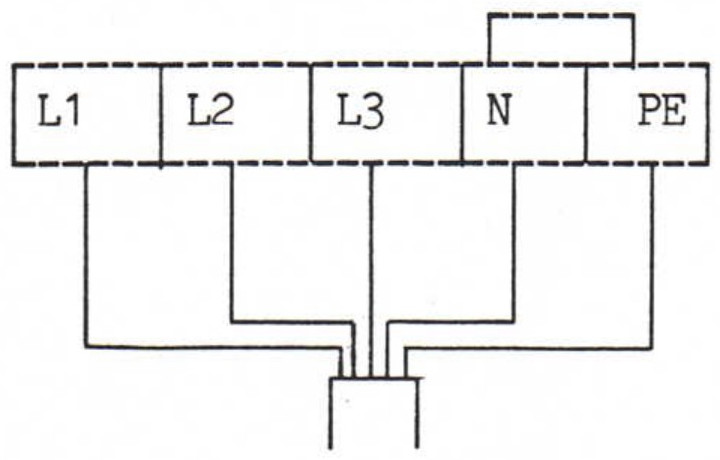
\includegraphics[width=\linewidth]{chapter1/electrical_connection_diagram.jpg}
        }
        \caption{Electrical connection diagram.} % Caption below the image
        \label{fig:electrical_connection} % Optional: add label for referencing
    \end{minipage}%
    \hfill % Add space between image and text
    \begin{minipage}[t]{\dimexpr\textwidth-8cm\relax} % Remaining width for the text
        \vspace{0pt} % Ensures top alignment of this minipage
        Total connection power: \dotfill 11 kVA \\\\
        Fuse, max.: \\
        200-220 V \dotfill 35 A \\
        380-500 V \dotfill 25 A
    \end{minipage}
\end{figure}

\begin{itemize}
    \item Switch off the main switch \textbf{-Q1-} on the control cabinet.
    \item Open the control cabinet door. Feed the connection cable through the \\provided opening and connect it to the input terminals L1, L2, L3, N, PE.
    \item For 4-pole connections, terminals N and PE must be bridged.
    \item Check the phase sequence using a phase sequence indicator on terminals L1, L2, L3. If necessary, swap two phases at the input terminals.
    \item Check all terminal screws on the terminal strips, contactors, relays, and fuses in the control cabinet for tightness.
    \item Only after establishing the correct phase sequence, switch on the main \\switch \textbf{-Q1-} on the control cabinet and perform a function test following the instructions on Page 3.01-1.
\end{itemize}

\notebox{NOTE}{The electrical documentation is located in a pocket on the inside of the control cabinet door and must remain in the machine!}

\notebox{CAUTION}{When connecting peripheral devices (reader-puncher, corner milling head, grinding head), check the voltage of the socket.}

Fuses must only be replaced with equivalent types.

Adjustment values on potentiometers, adjustment switches, machine parameters, etc., must only be changed by service personnel.

\section*{Commissioning Checklist}

Before starting the working spindles and axis movements, the following points must be completed:

\begin{enumerate}
    \item Proper setup, see page 1.03-1.
    \item Rust protection removed, see page 1.08-1.
    \item Oil bath filled, see page 1.09-1.
    \item Electrical connection, see page 1.10-1.
\end{enumerate}
\refstepcounter{chapter}
\addcontentsline{toc}{chapter}{General Description of the Machine}

\section{Technical Data}

\subsection{Work Area}
Adjustment of the cross support:
\begin{itemize}
    \item in the horizontal longitudinal axis (X-axis): \dotfill 400 mm
    \item in the vertical axis (Y-axis): \dotfill 375 mm
\end{itemize}

\noindent Adjustment of the spindle head:
\begin{itemize}
    \item in the horizontal transverse axis (Z-axis): \dotfill 250 mm
\end{itemize}

\subsection{Workspace}
Vertical mounting table \footnotemark[4]
\begin{itemize}
    \item Clamping surface: \dotfill 510 x 800 mm
    \item Number of guide grooves: \dotfill 1
\end{itemize}

\footnotetext[4]{Worktables, see Section 4 of the technical documentation.}

\subsection{Working Spindles}
\begin{itemize}
    \item Tool holder:\footnotemark[5] \dotfill ISO 40
    \item Quill stroke of the vertical working spindle: \dotfill 50 mm
    \item Clamping force of the tool clamp ISO-Type B Clamping pin: \dotfill N \footnotemark[6]
    \item MAHO-OTT Clamping groove: \dotfill N \footnotemark[6]
\end{itemize}

\footnotetext[5]{For tool holding according to DIN 69871, with pull studs ISO 7388, Type B.}
\footnotetext[6]{Tool clamping, see sheet 3.12-1; tool holders, see sheets 3.13-1 and 3.13-3.}

\subsection{Speeds and Feeds}
Working spindle speeds,\footnotemark[7] \\Directly programmable: \dotfill 80 - 4000 rpm

\footnotetext[7]{Transmission with 18 speed levels and a manual shifting step of 1.25, controlled by CNC and manually switchable.}

\vspace{.5cm}
\noindent Feeds, directly programmable: \footnotemark[8]
\begin{itemize}
    \item In the X, Y, Z axes: \dotfill 0.1 - 1500 mm/min
\end{itemize}

\footnotetext[8]{Minimum feed rate in axes X, Y, Z: 1 mm/min.}

\vspace{.2cm}
\noindent Rapid traverse:
\begin{itemize}
    \item In the X, Y, Z axes: \dotfill 2.5 m/min
\end{itemize}

\newpage
\subsection{Electrical Equipment}
\begin{itemize}
    \item Voltage: \dotfill 220/380 V \footnotemark[9]
    \item Frequency: \dotfill 50/60 Hz \footnotemark[9]
    \item Total connected load of the machine: \dotfill 11 kVA \footnotemark[9]
\end{itemize}

\footnotetext[9]{Standard configuration.}

\subsection{CNC Control\textsuperscript{\ref{fn:control}}}
\begin{itemize}
    \item Resolution of the linear measurement systems: \dotfill 0.001 mm
    \item Display of measured values: \dotfill Screen
    \item Number of simultaneously controlled axes: \dotfill 2
    \item Number of sequentially controlled axes: \dotfill 3
\end{itemize}

\footnotetext[10]{The CNC control is described in a separate manual.\label{fn:control}}

\subsection{Weight and Space Requirements}
Weight of the machine (with vertical milling head, \\
fixed table, and control cabinet), approx.:\dotfill 1,250 kg

\vspace{0.5cm}
\noindent Space requirements (without expansion dimensions):
\begin{itemize}
    \item Length: \dotfill 2,310 mm
    \item Width: \dotfill 2,475 mm
    \item Height: \dotfill 1,830 mm
\end{itemize}

\section{Machine Overview - Main Component Designation}

\begin{figure}[h]
    \centering
    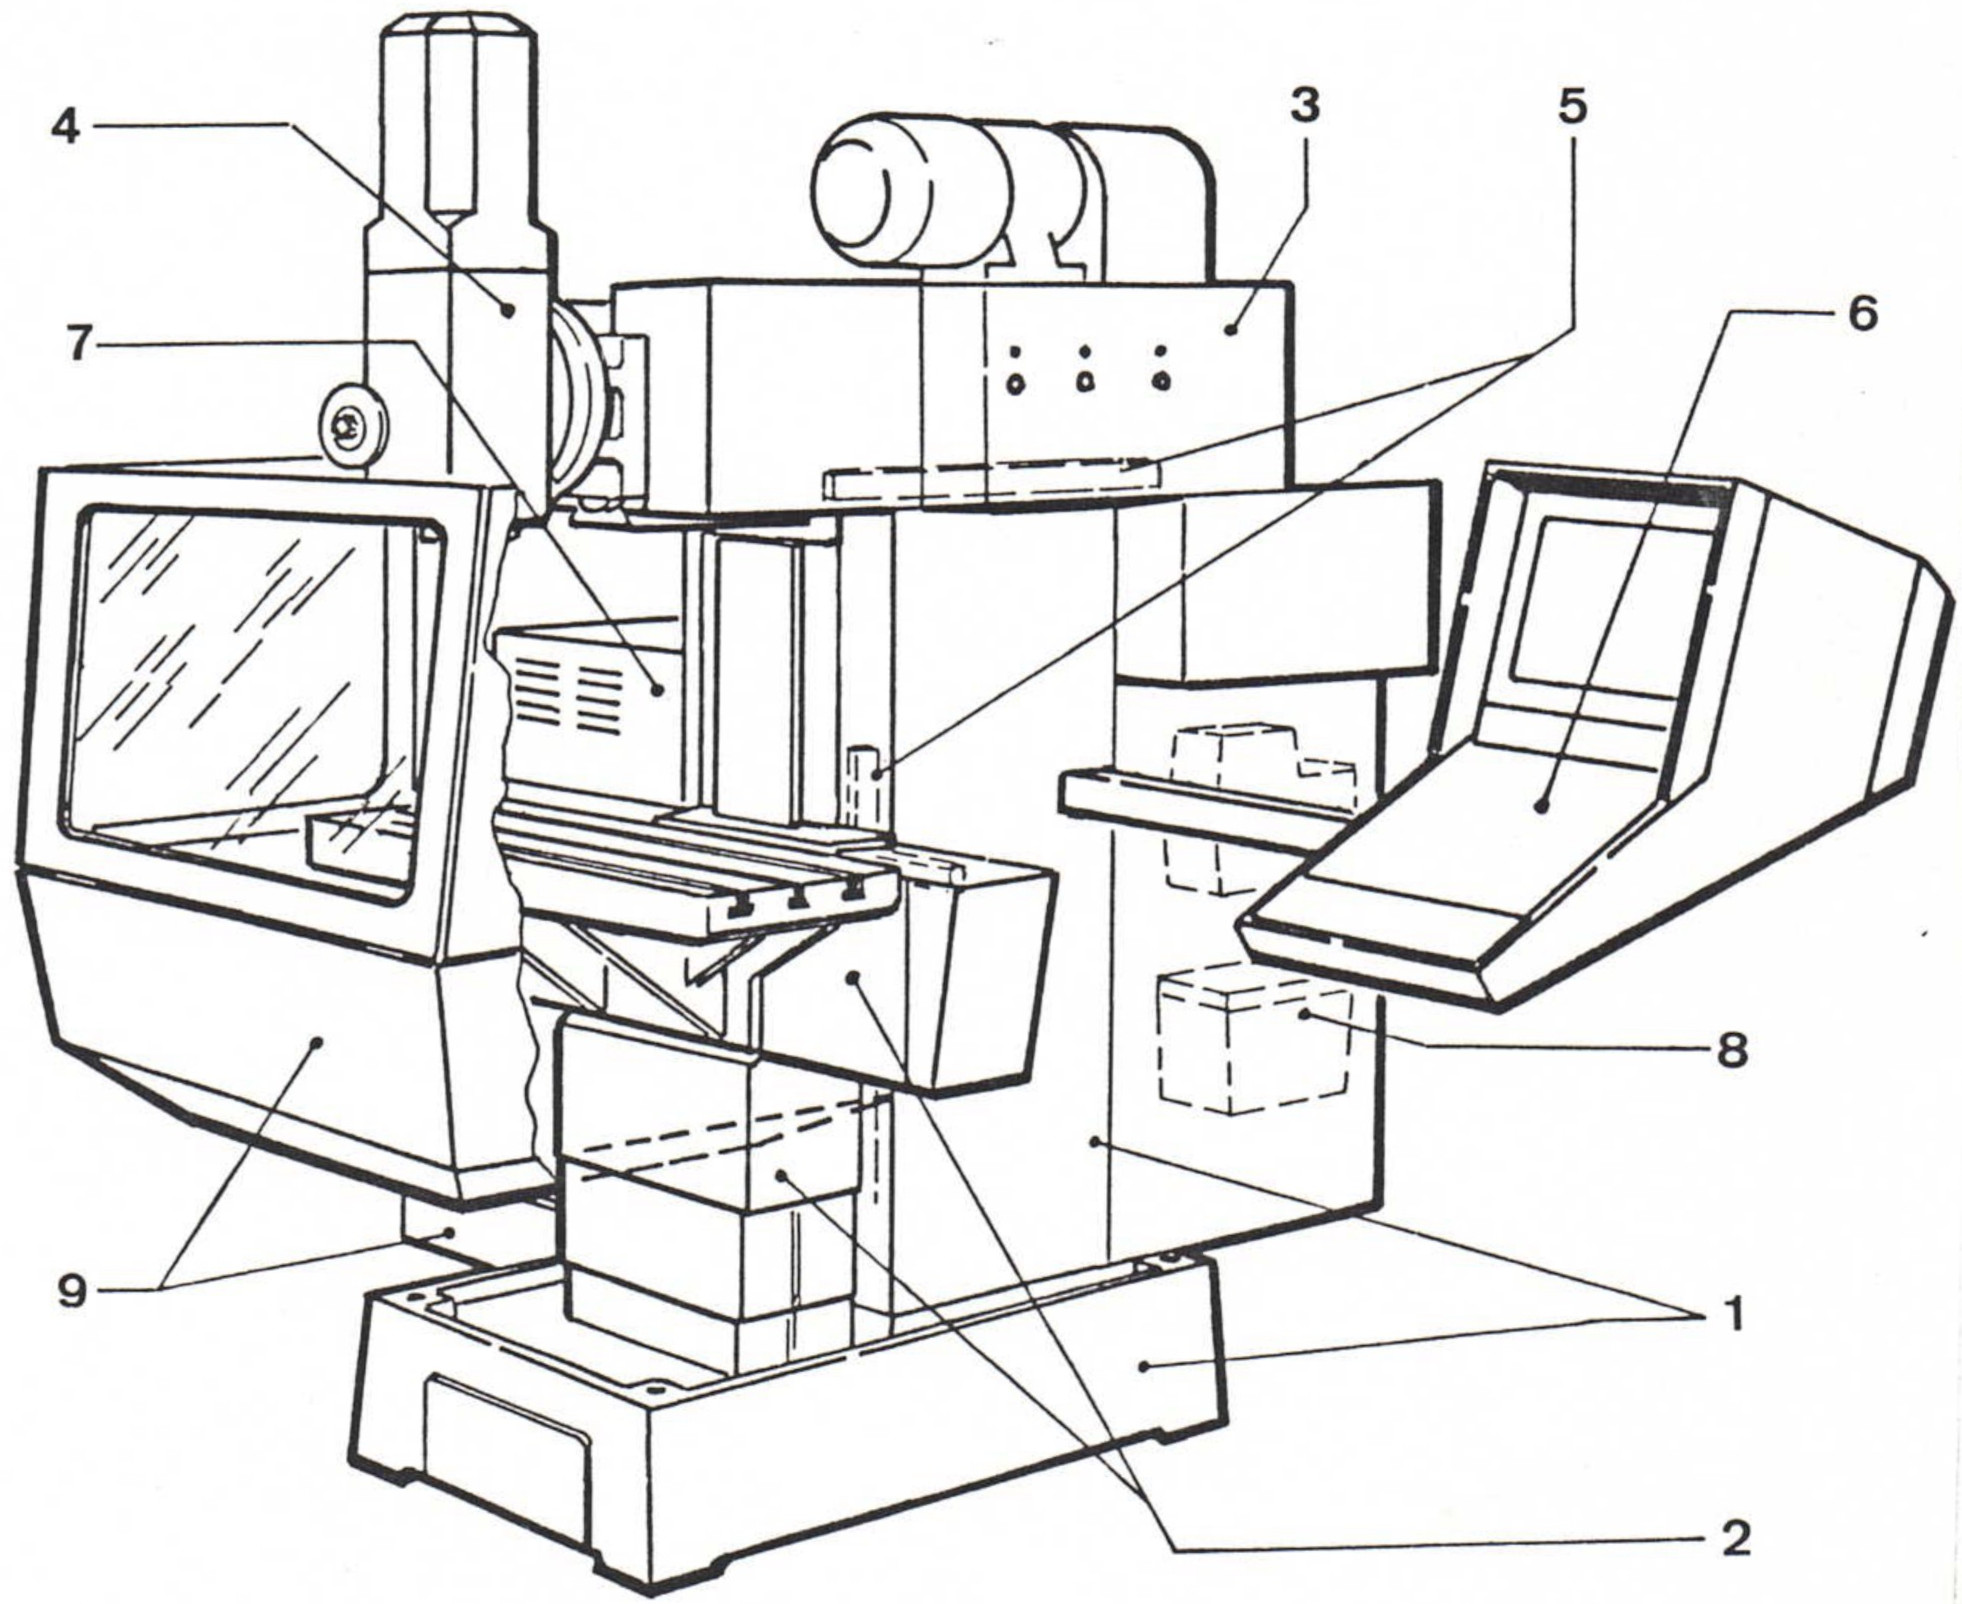
\includegraphics[width=0.8\textwidth]{chapter2/machine_overview.jpg}
    \caption{}
    \label{fig:machine_overview}
\end{figure}

\vspace{3cm}

\begin{enumerate}[itemsep=1pt,parsep=0pt]
    \item Machine stand with base and Y-axis feed drive
    \item Cross support with vertical mounting table and X-axis feed drive
    \item Spindle head with horizontal working spindle and Z-axis feed drive
    \item Vertical milling head with vertical working spindle
    \item Measuring systems
    \item CNC control
    \item Electrical system
    \item Central lubrication system / hydraulic system
    \item Coolant system / splash guard
\end{enumerate}

\notebox{NOTE}{Description of the operating elements for the worktables can be found in Section 4 of the operator's manual.}

\sectionLikeSubsection{Description of Machine Components}

\subsection{Machine Stand with Base}

\begin{figure}[h]
    \centering
    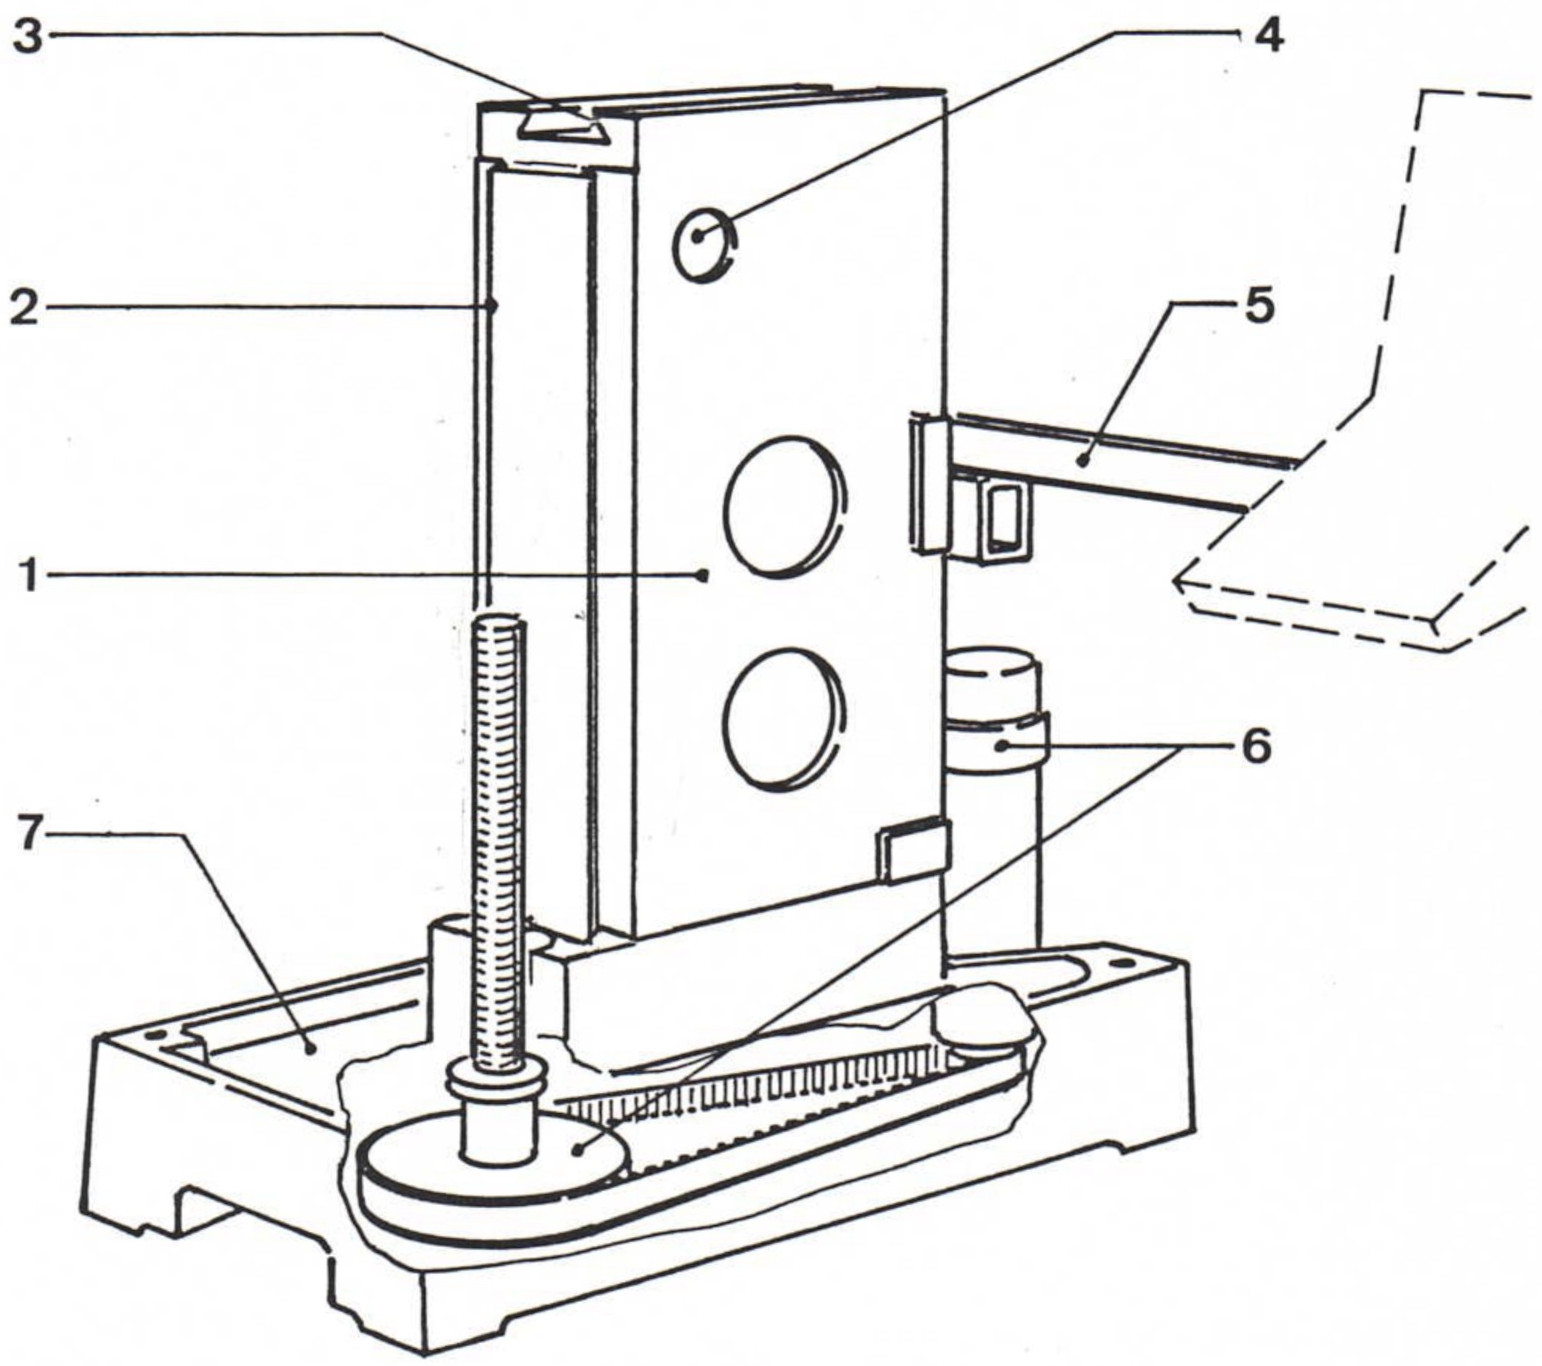
\includegraphics[width=0.6\textwidth]{chapter2/machine_stand.jpg}
    \caption{Diagram of the machine stand and its components.}
    \label{fig:machine_stand}
\end{figure}

\noindent The numbered components in the diagram are:
\begin{enumerate}[itemsep=1pt,parsep=0pt]
    \item Machine stand
    \item Dovetail guide for cross support
    \item Spindle head guide
    \item Opening for transporting the machine
    \item Swivel arm for control panel
    \item Y-axis feed drive
    \item Stand base
\end{enumerate}

\noindent The machine stand (1) with stand base (7) serves as the structural support for the other assemblies.

\vspace{.3cm}

\noindent The dovetail guide (2) on the front allows the vertical slide of the cross support to move smoothly.

\vspace{.3cm}

\noindent The mating surfaces of the spindle head (3) on the upper section of the \\machine stand are coated with the same plastic sliding material as the mating surface of the cross support.

\vspace{.3cm}

\noindent In the upper half of the stand, there is a continuous opening (4) designed to accommodate the transport rod.

\vspace{.3cm}

\noindent The Y-axis feed drive (6) is housed within the stand base (7).

\vfill
\clearpage

\subsection{Cross Support}

\begin{minipage}{0.5\textwidth}
    \begin{enumerate}[itemsep=1pt,parsep=0pt]
        \item Longitudinal slide
        \item Vertical slide, Y-axis
        \item DC motor, Y-axis
        \item Timing belt, Y-axis
        \item Ball screw, Y-axis
        \item Dovetail guide, Y-axis
        \item Ball screw, X-axis
        \item Timing belt, X-axis
        \item DC motor, X-axis
        \item Dovetail flat guide, X-axis
    \end{enumerate}
\end{minipage}%
\begin{minipage}{0.5\textwidth}
    \centering
    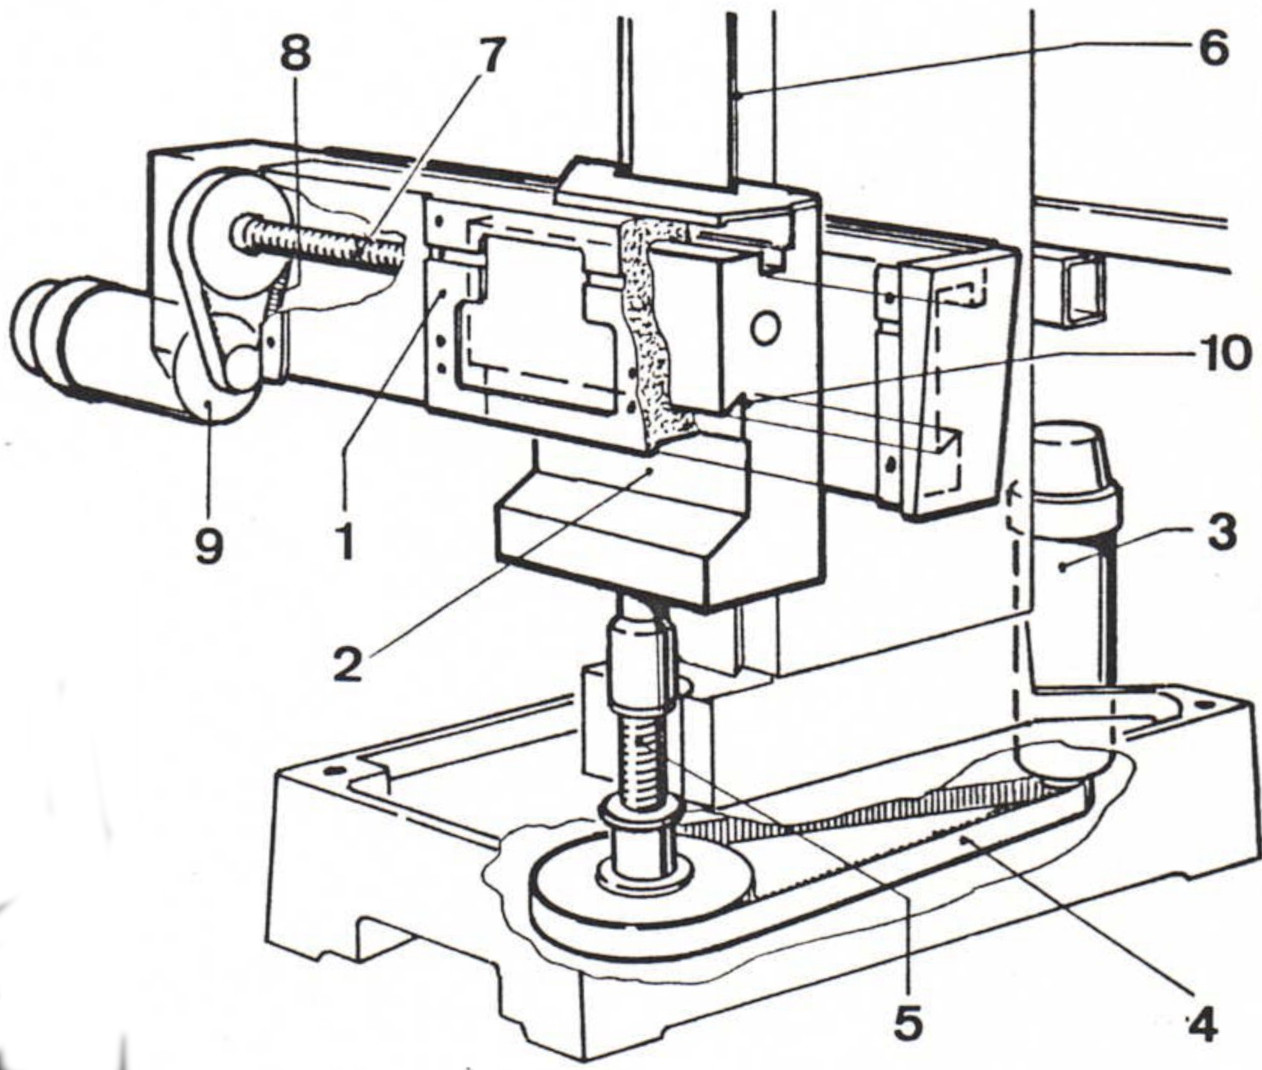
\includegraphics[width=0.9\textwidth]{chapter2/cross_support.jpg}
    \captionof{figure}{}
    \label{fig:cross_support}
\end{minipage}

\vspace{1cm}

\noindent The cross support carries out the necessary longitudinal and vertical\\ movements for workpiece machining.

\vspace{.3cm}

\noindent It consists of the longitudinal slide "vertical mounting table" (X-axis) (1) and the vertical slide (Y-axis) (2).

\vspace{.3cm}

\noindent The worktables are mounted on the vertical mounting table; see Chapter 4.

\vspace{.3cm}

\noindent A DC motor (3), along with timing belts (4) and a ball screw (5), provides the feed drive for the Y-axis.

\vspace{.3cm}

\noindent The vertical slide moves along the dovetail guide (10) on the machine stand. The mating surfaces on the support are coated with a plastic sliding material that has excellent wear resistance, emergency running properties, damping characteristics, and friction performance, allowing smooth sliding \\(eliminating the stick-slip effect).

\vspace{.3cm}

\noindent The longitudinal slide is guided by the vertical slide using a dovetail guide (6). Its mating surfaces are also coated with the specialized sliding \\material.

\vspace{.3cm}

\noindent All guides are equipped with wipers to protect against chips, dirt, and \\coolant contamination and are automatically lubricated via a central \\lubrication system.

\vspace{.3cm}

\noindent The longitudinal slide (X-axis) is driven by a DC motor (9) through a timing belt (8) and a ball screw (7).

\vfill
\clearpage

\subsection{Spindle Head}

\begin{minipage}{0.5\textwidth}
    \begin{enumerate}[itemsep=1pt,parsep=0pt]
        \item Spindle head housing
        \item Main motor
        \item Gearbox
        \item Poly V-belt
        \item Timing belt
        \item DC motor, Z-axis
        \item Ball screw
        \item Horizontal working spindle
        \item Vertical milling head drive shaft
    \end{enumerate}
\end{minipage}%
\begin{minipage}{0.5\textwidth}
    \centering
    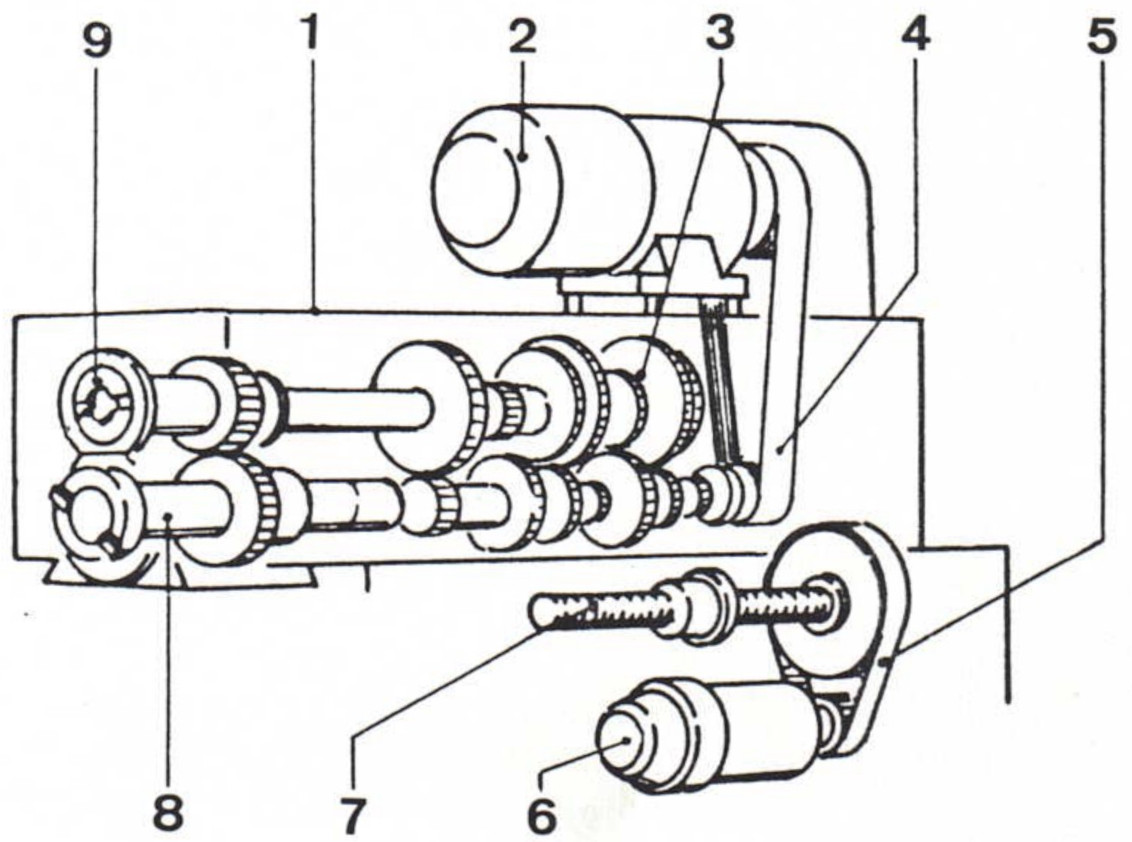
\includegraphics[width=0.9\textwidth]{chapter2/spindle_head.jpg}
    \captionof{figure}{}
    \label{fig:spindle_head}
\end{minipage}

\vspace{1cm}

\noindent The spindle head (1) is equipped with a dovetail guide and is mounted on the upper side of the machine stand.

\vspace{.3cm}

\noindent Its front side accommodates either the vertical milling head or the \\counterholder for horizontal milling (see also pages 3.05-1, 3.07-1 to \\3.09-1).

\vspace{.3cm}

\noindent The dovetail guide is fitted with wipers to prevent the ingress of chips, dirt, and coolant.

\vspace{.3cm}

\noindent The mating surfaces on the machine stand are coated with the same specialized sliding material as those on the cross support.

\vspace{.3cm}

\noindent The three-phase main motor (2) is mounted on top of the spindle head.

\vspace{.3cm}

\noindent The main motor's torque is transmitted via a poly V-belt (4) and an integrated 18-speed gearbox (3) within the spindle head to the working spindle (8).

\vspace{.3cm}

\noindent The working spindle (8) runs in five preloaded precision spindle bearings, which are permanently lubricated for maintenance-free operation.

\vspace{.3cm}

\noindent A DC motor (6) mounted beneath the spindle head, together with the timing belt (5) and ball screw (7), drives the Z-axis feed motion.

\vfill
\clearpage

\subsection{Vertical Milling Head}

\begin{minipage}{0.5\textwidth}
    \begin{enumerate}[itemsep=1pt,parsep=0pt]
        \item Spindle head
        \item Milling head extension arm
        \item Intermediate flange
        \item Milling head housing
        \item Vertical working spindle
        \item Quill adjustment mechanism
    \end{enumerate}
\end{minipage}%
\begin{minipage}{0.5\textwidth}
    \centering
    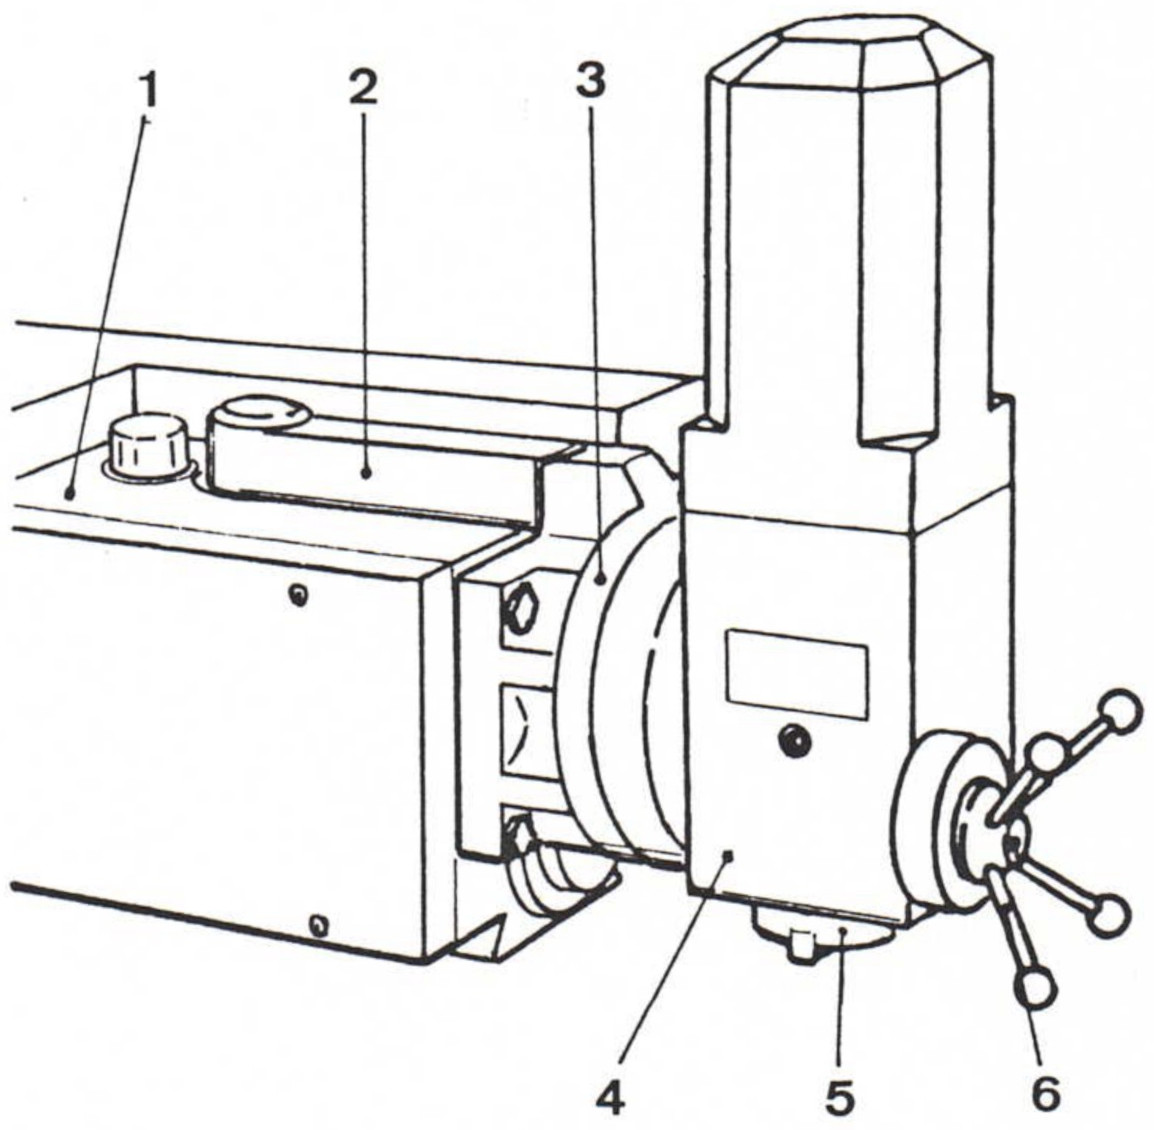
\includegraphics[width=0.9\textwidth]{chapter2/vertical_milling_head.jpg}
    \captionof{figure}{}
    \label{fig:vertical_milling_head}
\end{minipage}

\vspace{1cm}

\noindent The vertical milling head is mounted on top of the spindle head (1) with a pivotable extension arm. This allows it to be swung out of the working area when not in use.

\vspace{.3cm}

\noindent The milling head housing (4) is mounted on the intermediate flange (3) and can be swiveled 90° in both directions.

\vspace{.3cm}

\noindent The vertical working spindle (5) is supported by four preloaded precision spindle bearings within a quill. Due to its lifetime lubrication, these bearings are maintenance-free.

\vspace{.3cm}

\noindent The quill can be extended using the quill adjustment mechanism (6).

\vspace{.3cm}

\noindent Detailed instructions on operation and handling can be found on pages 3.07-1 to 3.09-1.

\newpage
\subsection{Measuring Systems}

The measuring systems operate contact-free and maintenance-free, with a \\resolution of 0.001 mm. Protective covers shield them from the ingress of chips and coolant.

\vspace{0.3cm}

\noindent A detailed functional description of the measuring systems can be found in Chapter 5.

\vspace{0.3cm}

\noindent The X-axis measuring system is installed at the top of the cross support.

\vspace{0.3cm}

\noindent The Y-axis measuring system is located on the left side of the machine stand.

\vspace{0.3cm}

\noindent The Z-axis measuring system is mounted on the left side of the spindle head.

\vspace{0.3cm}

\noindent Thermal expansion of the spindle head, caused by the working spindle heating up, is compensated by the Z-axis measuring system.

\vspace{0.3cm}

\noindent To ensure high measurement accuracy, an invar rod (2) fixed to the spindle head compensates for thermal expansion by adjusting the scale bar (4), \\maintaining precise measurements throughout the machine's operational life.

\vspace{0.5cm}

\noindent\textbf{\uline{Z-Axis Measuring System}}

\begin{figure}[h]
    \centering
    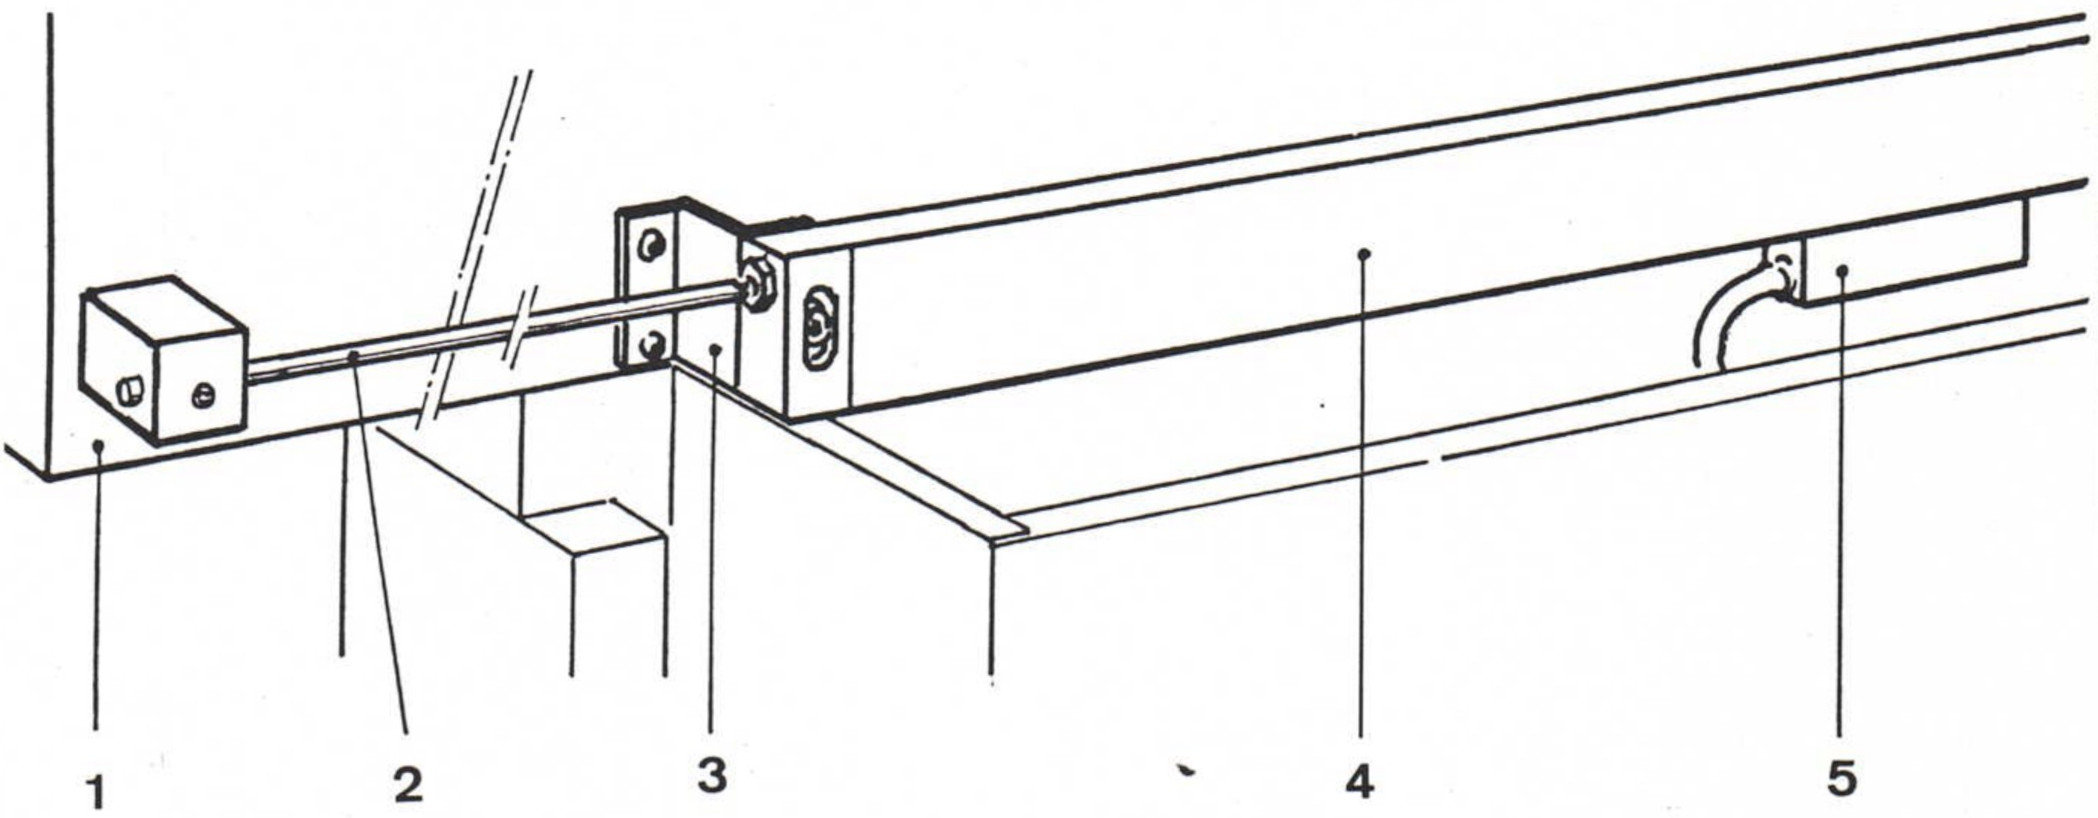
\includegraphics[width=0.9\textwidth]{chapter2/measuring_system_z_axis.jpg}
    \caption{}
    \label{fig:measuring_system_z}
\end{figure}

\begin{enumerate}[itemsep=1pt,parsep=0pt]
    \item Spindle head
    \item Invar rod
    \item Suspension strips
    \item Scale bar, Z-axis
    \item Measuring head
\end{enumerate}

\newpage

\subsection{CNC Control 432 E/Graphics}

The CNC control unit is housed in the control cabinet (5), while the control panel (2) and screen (3) are mounted in a control console. This console (4) is rotatable and is attached to a swivel arm (1) on the left side of the machine.

\vspace{0.3cm}

\noindent The construction, function, and programming of the control system are \\described in the CNC 432/10-Graphics manual.

\vspace{-.3cm}


\begin{minipage}[b]{0.5\textwidth}
    \textbf{\uline{CNC Control 432 E/Graphics}}
    \begin{enumerate}[itemsep=1pt,parsep=0pt]
        \item Swivel arm
        \item Control panel
        \item Screen
        \item Control console
    \end{enumerate}
\end{minipage}%
\begin{minipage}{0.5\textwidth}
    \centering
    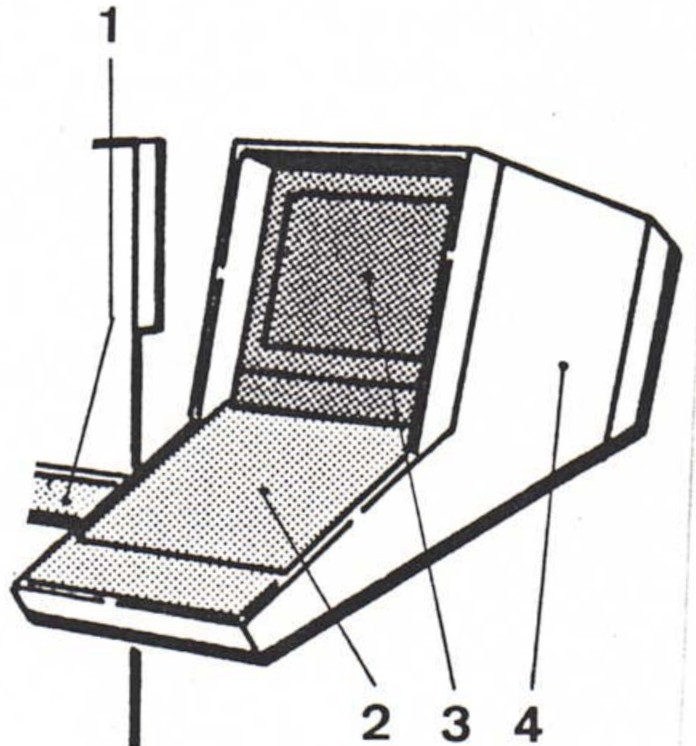
\includegraphics[width=0.6\textwidth]{chapter2/cnc_control.jpg}
    \captionof{figure}{}
    \label{fig:cnc_control}
\end{minipage}

\vspace{-1cm}

\subsection{Electrical System}

The control cabinet (5), located at the rear of the machine, contains the power module, which supplies energy to the machine’s drives.

\vspace{0.3cm}

\noindent It processes signals from the CNC 432 E control, regulates the drives, and protects against overcurrent.

\vspace{0.3cm}
\noindent Inside the control cabinet door (8) are the main switch (9) and the adjustment module (10).

\begin{minipage}[c]{0.45\textwidth}
    \begin{enumerate}[itemsep=1pt,parsep=0pt]
        \setcounter{enumi}{4}
        \item Control cabinet
        \item Transformer room
        \item Heat exchanger
        \item Control cabinet door
        \item Main switch
        \item Adjustment module
        \item CNC Control 432 E/Graphics
    \end{enumerate}

    \noindent The adjustment module contains the following switches:
\end{minipage}%
\begin{minipage}{0.6\textwidth}
    \centering
    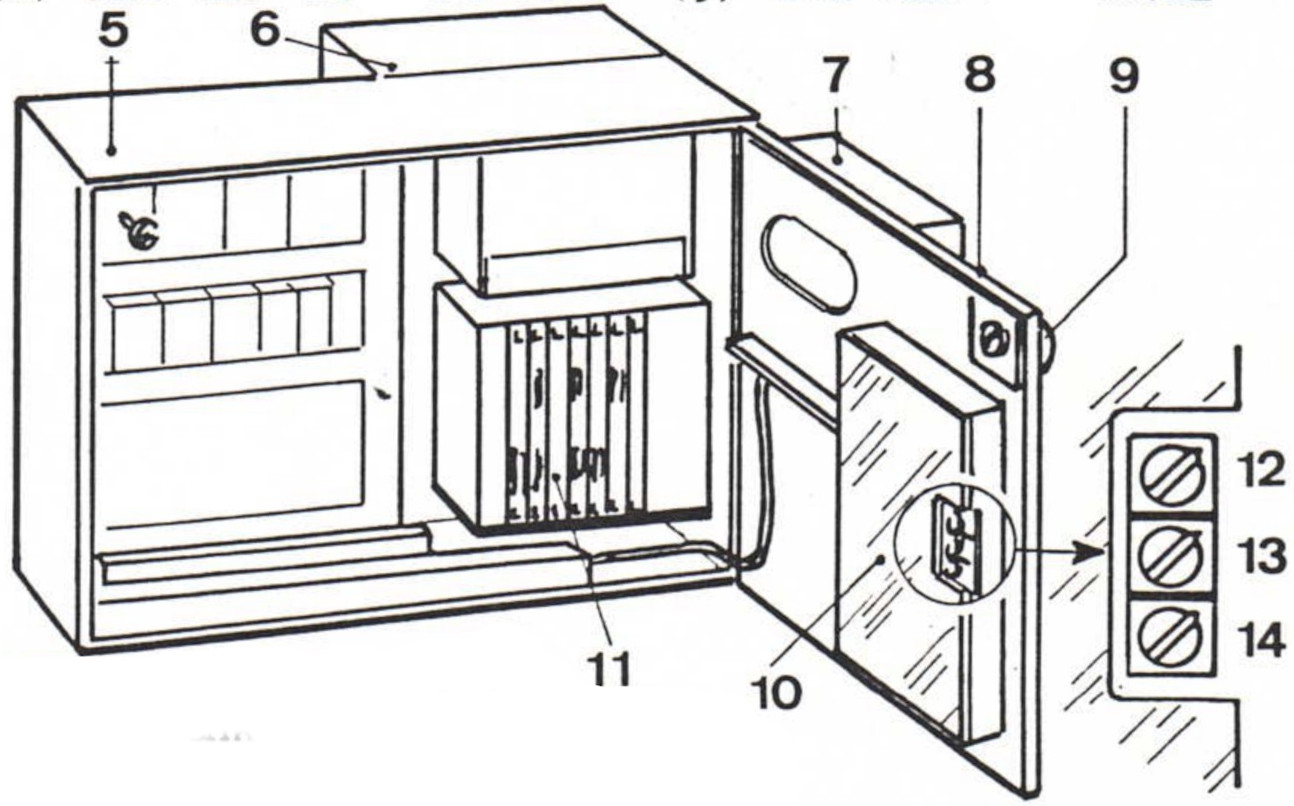
\includegraphics[width=\textwidth]{chapter2/electrical_system.jpg}
    % \captionof{figure}{}
    \label{fig:electrical_system}
\end{minipage}

\begin{textblock*}{\textwidth}(3cm, 21cm)  % Adjust coordinates as needed
    \begin{enumerate}[itemsep=1pt,parsep=0pt]
        \setcounter{enumi}{11}
        \item \textbf{Rotary switch (7S1):} "Brake Y-axis engaged/disengaged"
        \item \textbf{Rotary switch (19S1):} "Read machine constants"
        \item \textbf{Rotary switch (19S2):} "Test operation"
    \end{enumerate}
\end{textblock*}

\vspace{2cm}

\notebox{NOTE}{The numbers in parentheses correspond to circuit diagram labels.}

\section{Movement Directions}

\begin{figure}[h]
    \centering
    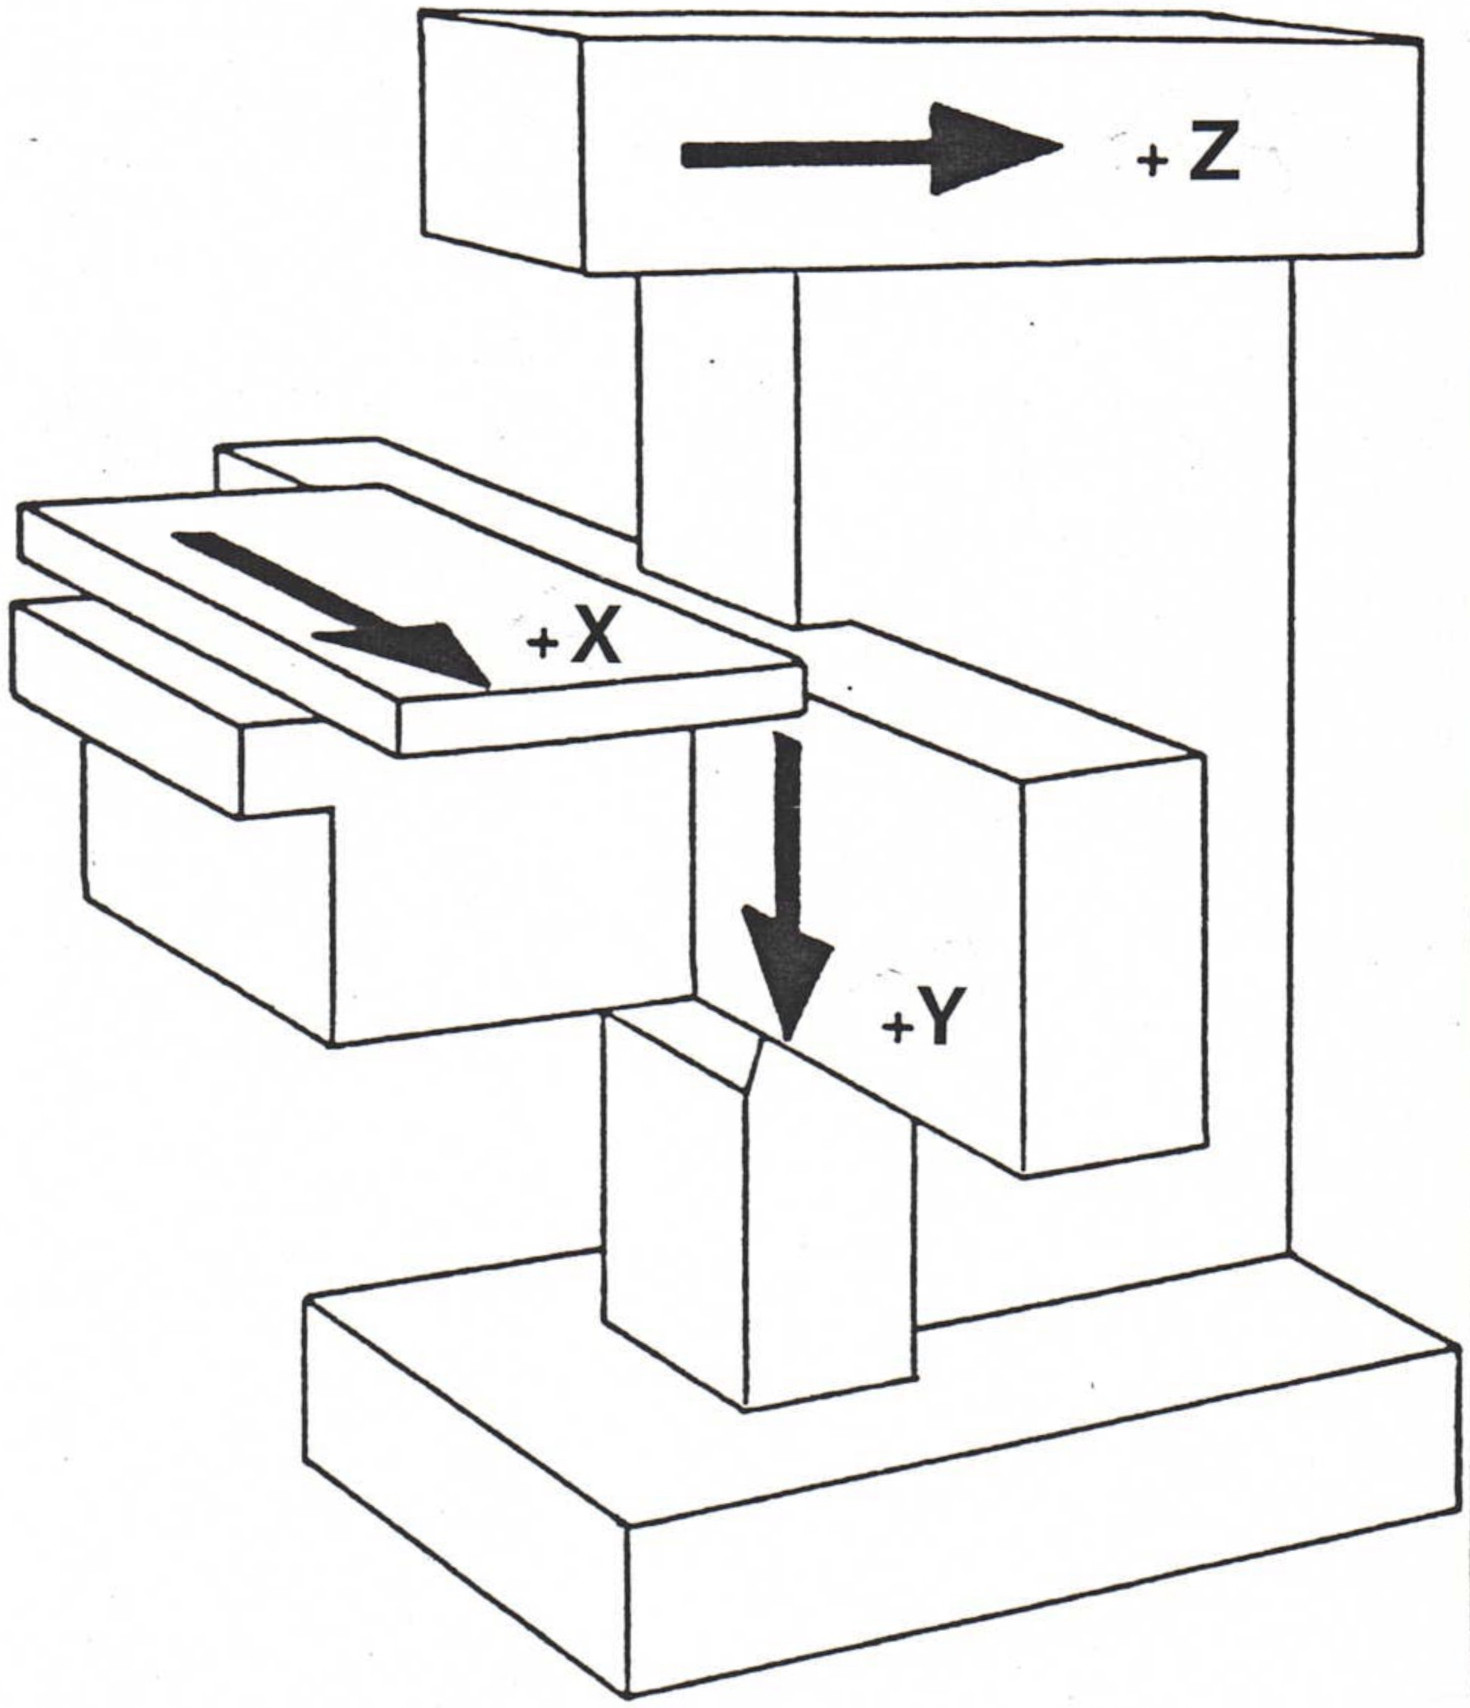
\includegraphics[width=0.8\textwidth]{chapter2/movement_directions.jpg}
\end{figure}

\vspace{0.5cm}

\noindent \textbf{Axis Definitions:}

\vspace{0.3cm}

\noindent \begin{tabular}{ l l }
\textbf{X-Axis} & Horizontal longitudinal movement of the vertical mounting table: \\
                & Left \enquote{-} or Right \enquote{+}. \\
\textbf{Y-Axis} & Vertical movement of the cross support: \\
                & Up \enquote{-} or Down \enquote{+}. \\
\textbf{Z-Axis} & Horizontal transverse movement of the spindle head: \\
                & Forward \enquote{-} or Backward \enquote{+}. \\
\end{tabular}

\section{Control Station (Machine)}

\begin{figure}[h]
    \centering
    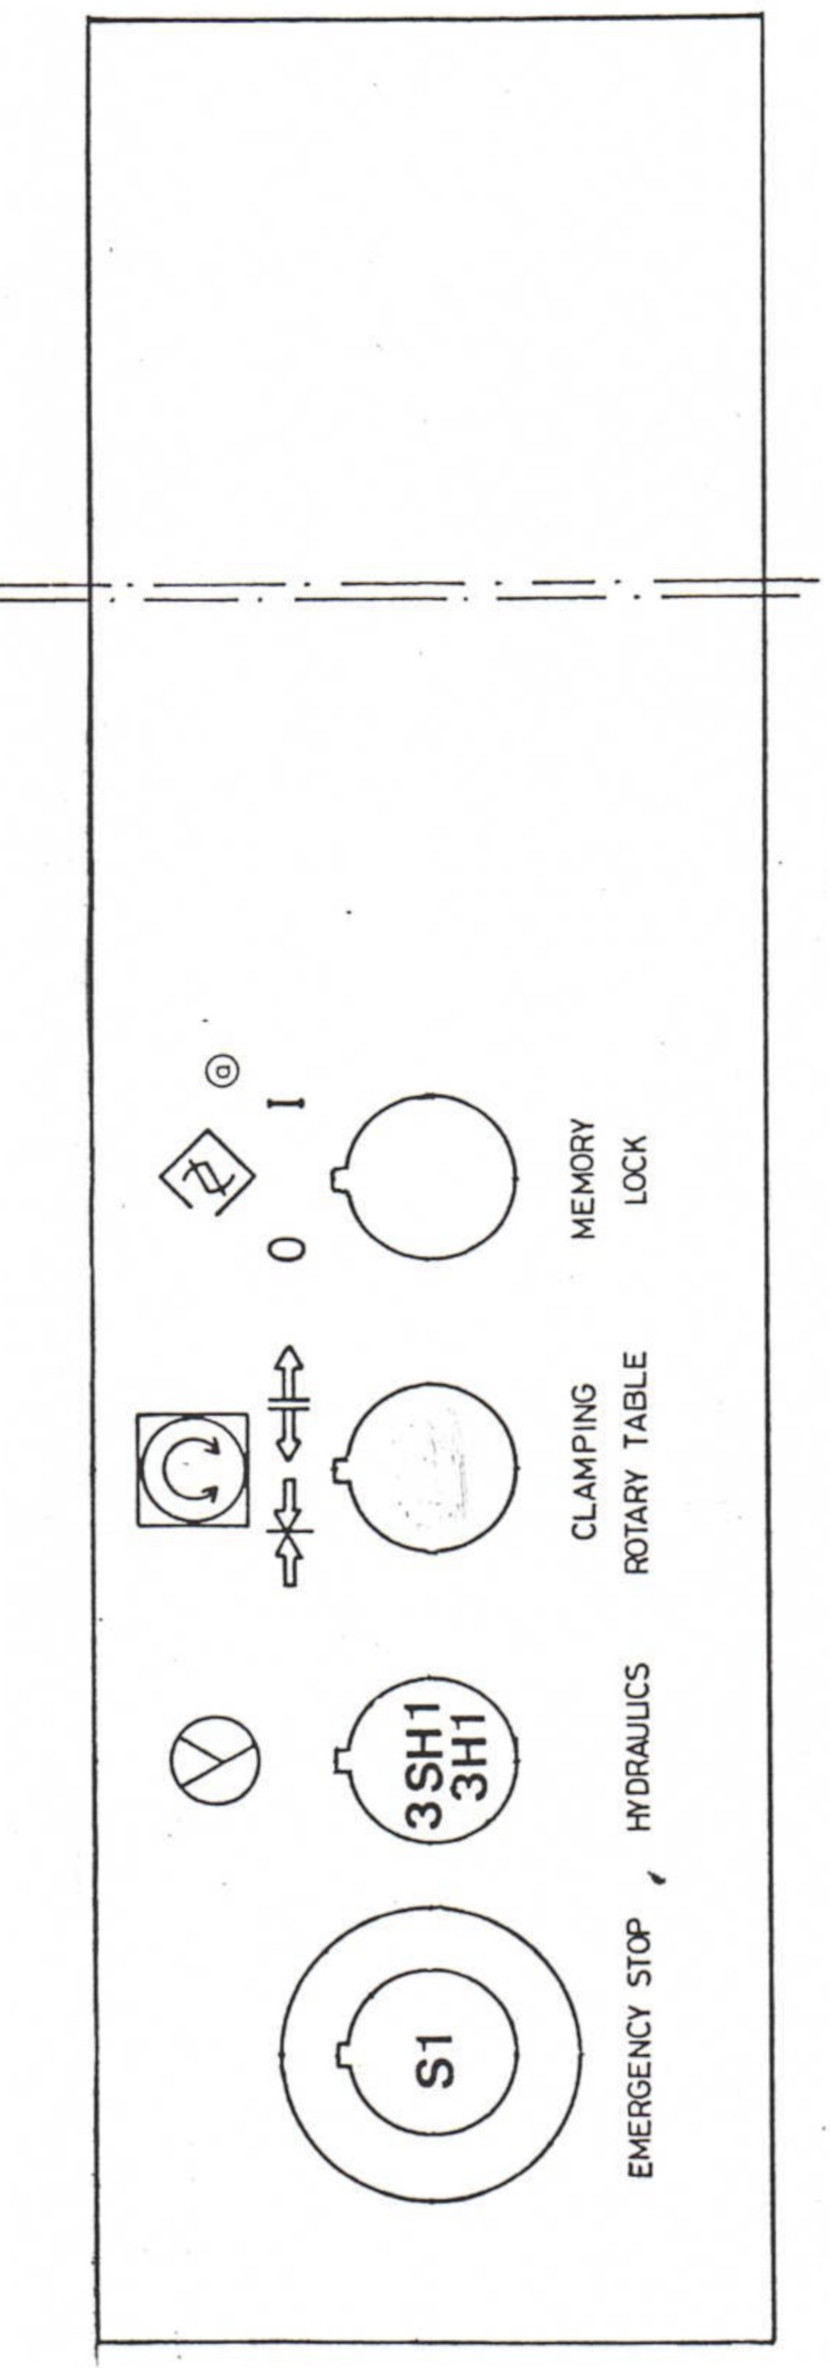
\includegraphics[width=0.38\textwidth]{chapter2/control_station.jpg} % Replace with actual filename
\end{figure}

\sectionLikeSubsection{Control Station - Function of the Operating Elements (Machine)}

\vspace{0.3cm}

\noindent % Remove paragraph indentation
\begin{tabular}{|c|l|p{10cm}|}
    \hline\hline
    \textbf{Nr.} & \textbf{Operating Element} & \textbf{Function} \\
    \hline\hline
    -S1-   & Emergency stop button & Emergency stop. All machine motors are immediately shut down.\footnotemark[11] \\
    \hline
    -3SH1- & Illuminated push button & Hydraulics, central lubrication, and control ON. \\
    -3H1-  & Indicator light & ON. \\
    \hline\hline
\end{tabular}

\vspace{0.5cm}

\footnotetext[11]{After activation, the red emergency stop button remains locked. Before restarting the machine, the locking mechanism must be released by turning the emergency stop button to the right.}

\setcounter{page}{4}

\sectionLikeSubsection{Handheld Control Unit}

\noindent
For ease of setup when machining a workpiece, the CNC 432 control system is also equipped with a handheld control unit. It enables the operation of the following functions:

\begin{itemize}[itemsep=1pt,parsep=0pt]
    \item Axis selection in positive or negative direction for each axis. Operating modes: SINGLE, AUTOMATIC, MANUAL
    \item Program creation via PLAY-BACK
    \item Machine status
    \item Feed rate control (potentiometer)
    \item Spindle feed HOLD
    \item Feed START
    \item Coolant ON/OFF
    \item Tool clamp RELEASE/CLAMP
    \item EMERGENCY STOP
\end{itemize}

\noindent
Safety activation is required for enabling the keyboard from the handheld control unit for safety reasons.

\vspace{0.3cm}

\notebox{NOTE}{For operation with the handheld control unit, see the separate CNC 432/Graphics operating manual.}

\vspace{0.3cm}

\notebox{WARNING}{On \enquote{E}-machines, the following keys are \uline{not activated}:}

\vspace{-0.6cm}

\begin{center}
    \fbox{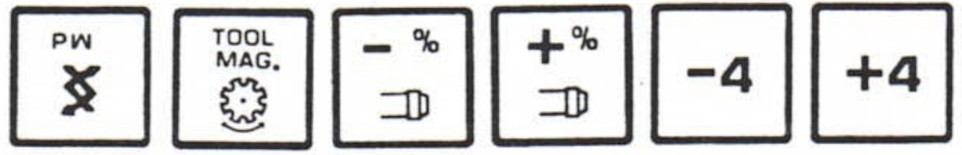
\includegraphics[width=0.4\textwidth]{chapter2/deactivated_keys.jpg}}
\end{center}

\vspace{-0.5cm}

\begin{figure}[h]
    \centering
    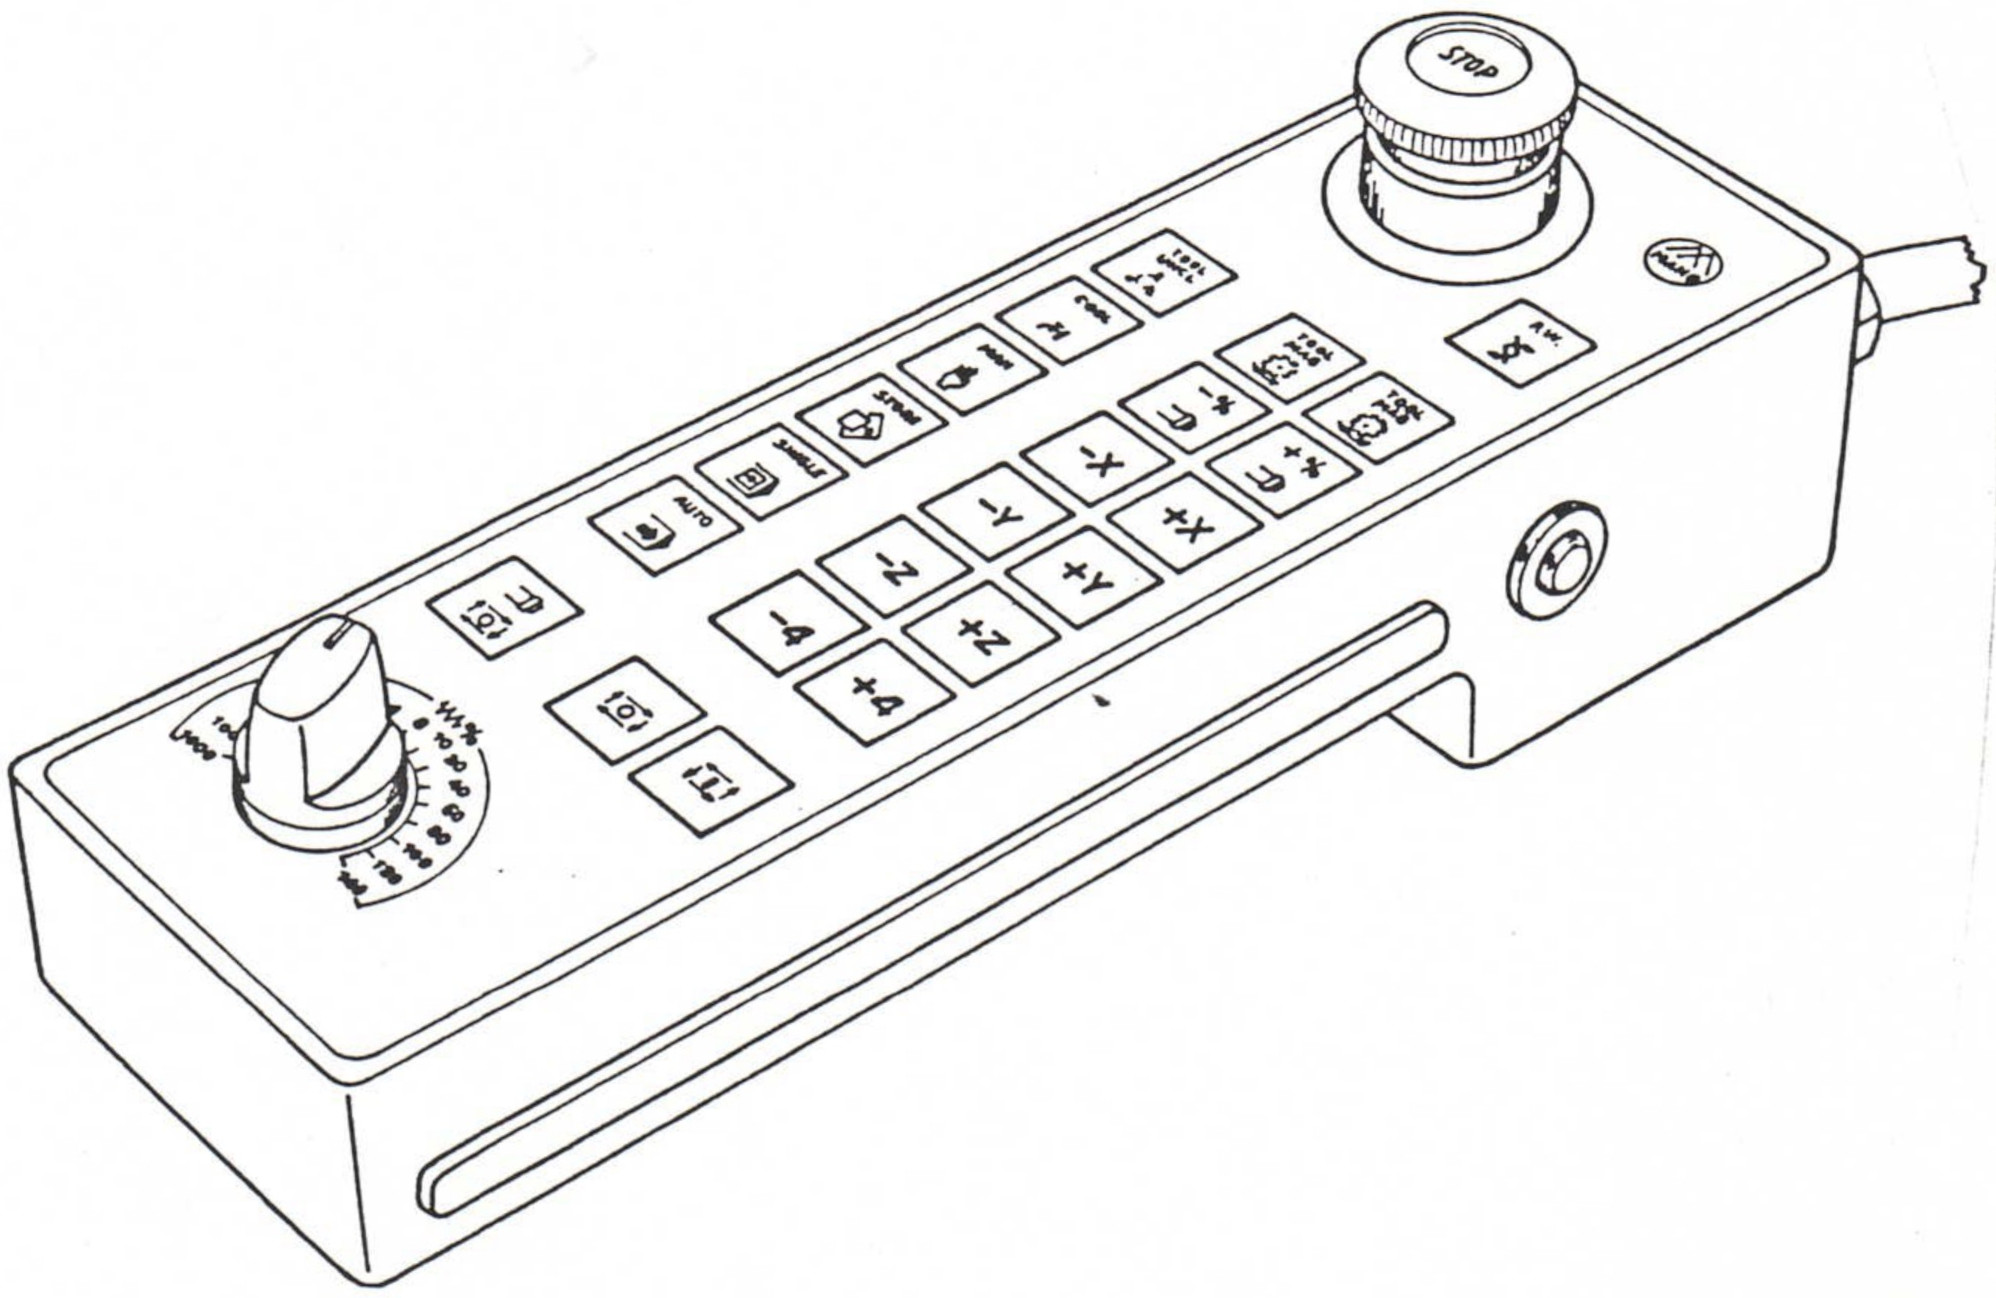
\includegraphics[width=0.9\textwidth]{chapter2/handheld_control.jpg}
\end{figure}

\section{Gear Train Schematic}
\setcounter{section}{10}
\begin{minipage}{\textwidth}
    \begin{adjustwidth}{-2cm}{-3cm}
        \centering
        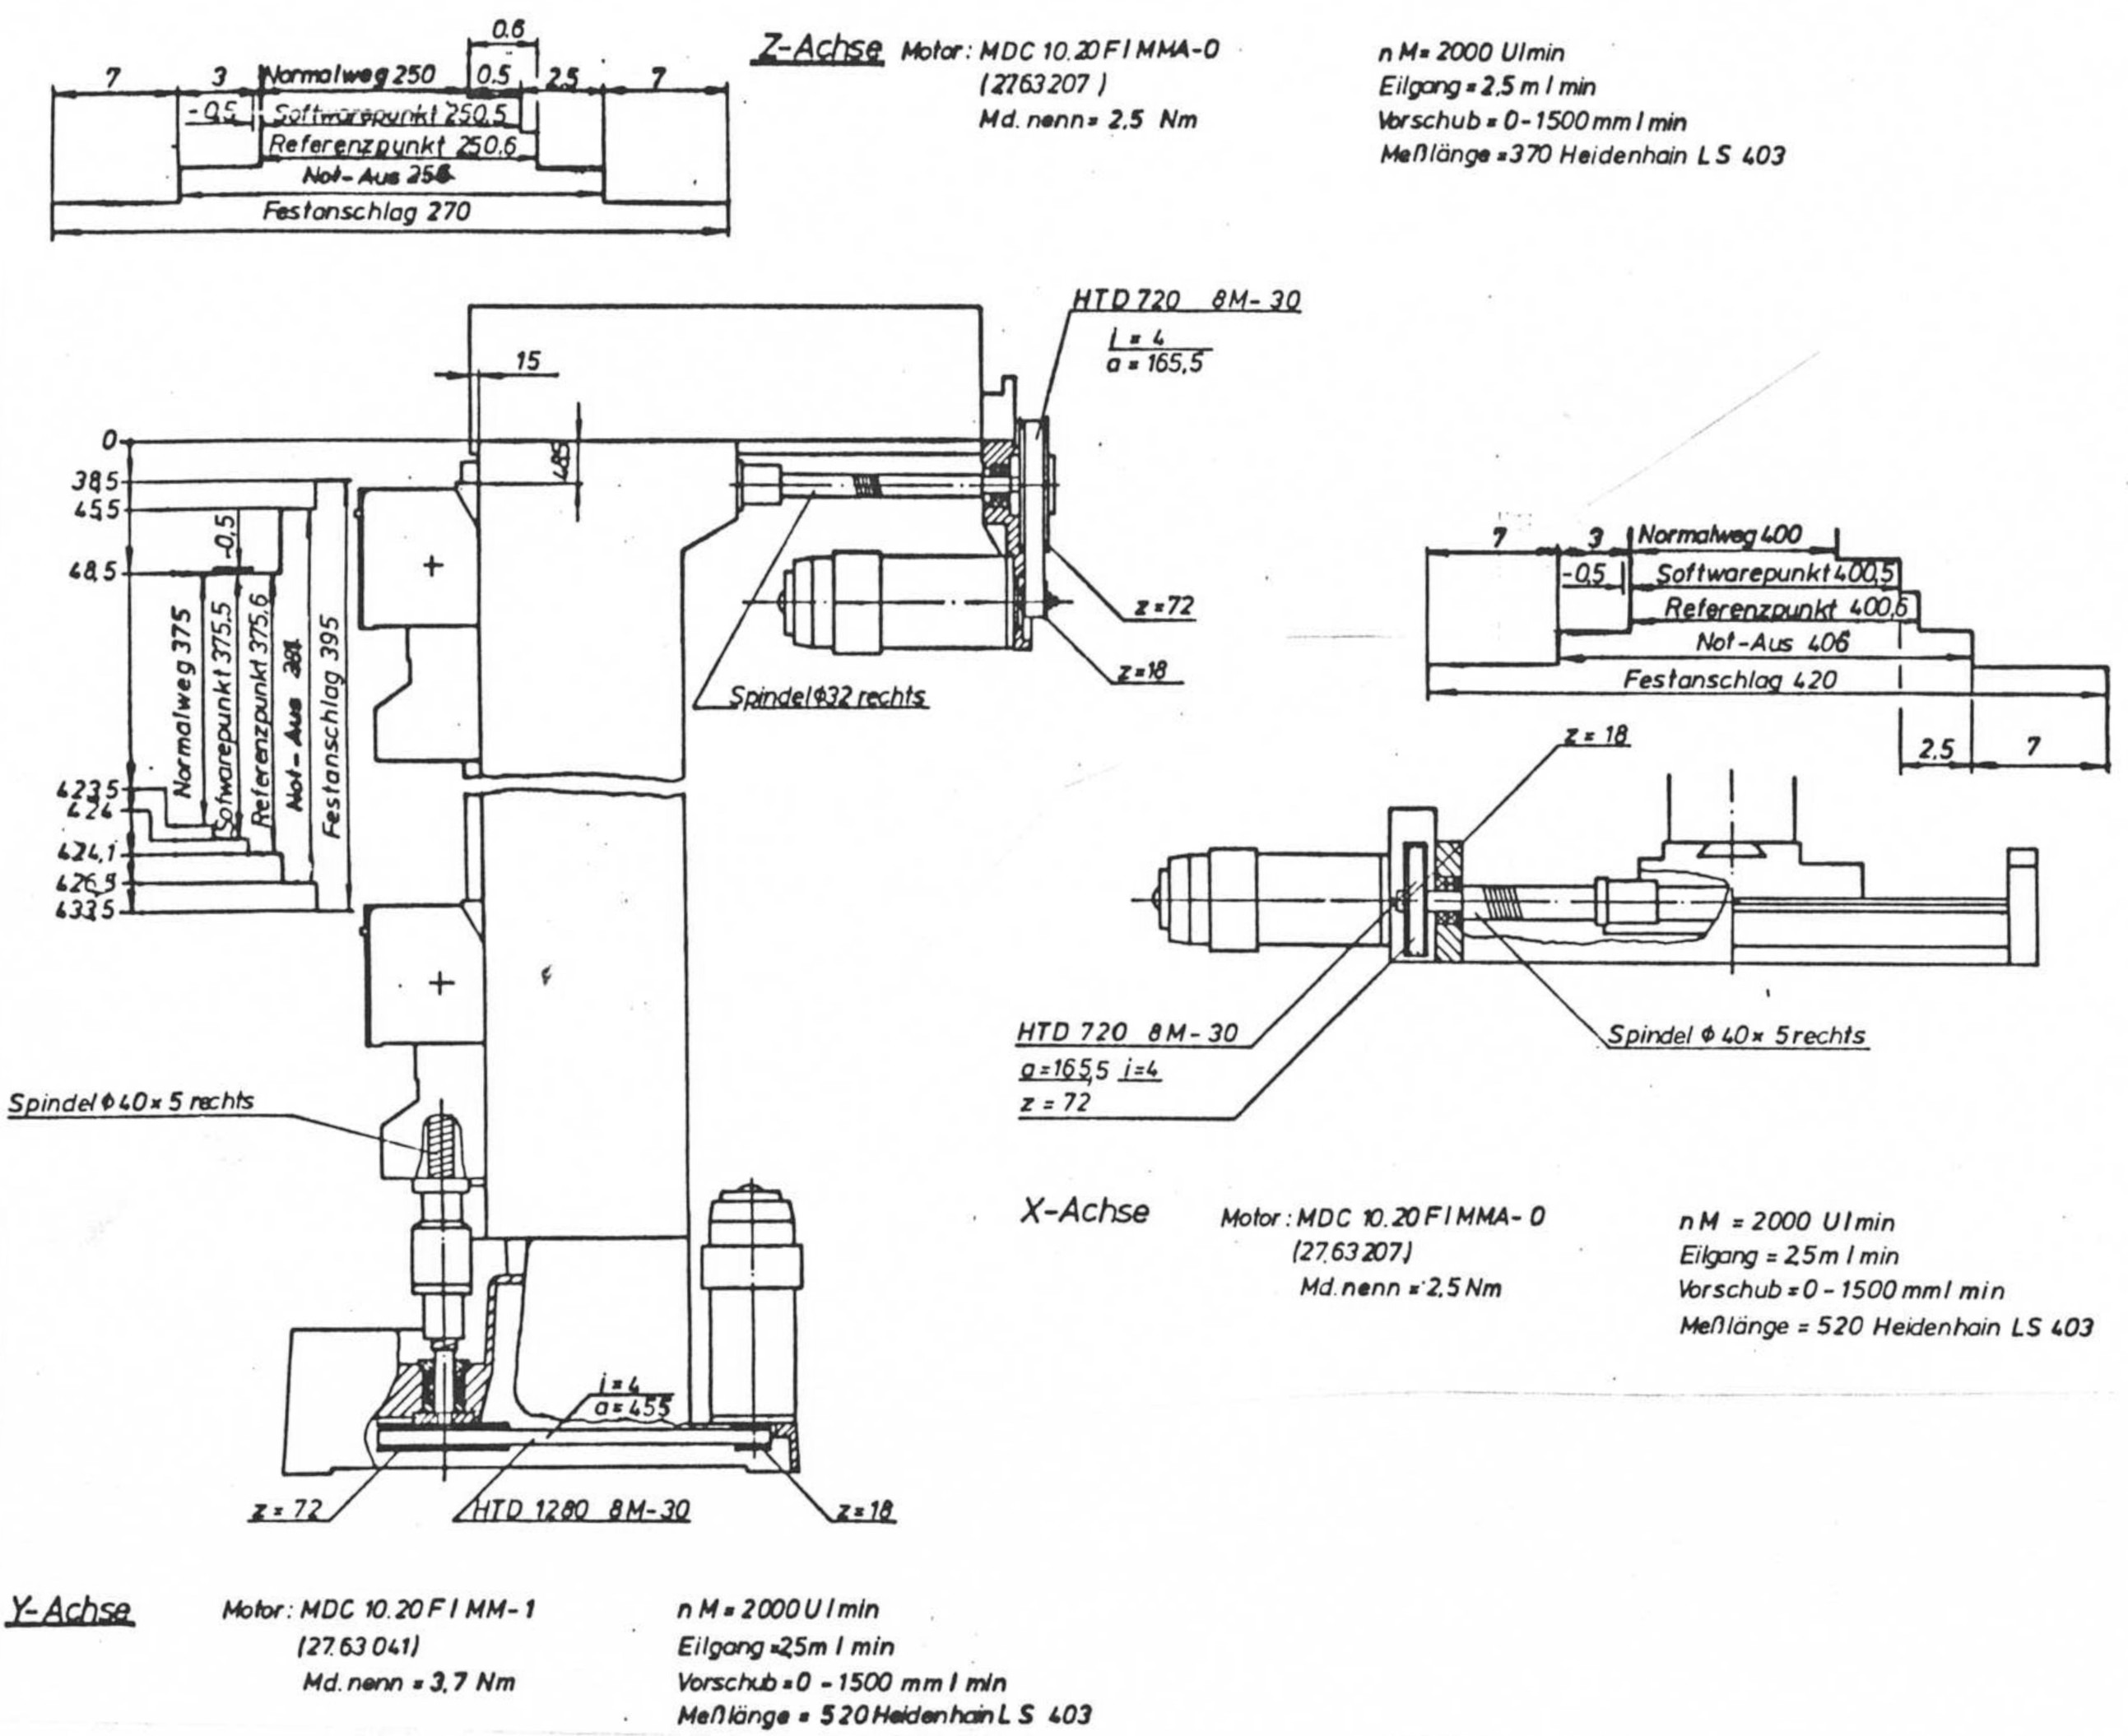
\includegraphics[angle=90,height=.9\textheight]{chapter2/gear_train_schematic.jpg}
    \end{adjustwidth}
    \label{fig:gear_train}
\end{minipage}

\sectionLikeSubsection[\texorpdfstring{14.48805/14.488111 (50/60Hz)}{14.48805-14.488111}]%
{Gear Train Schematic - Main Gearbox}

\vspace{-.5cm}

\begin{figure}[h]
    \centering
    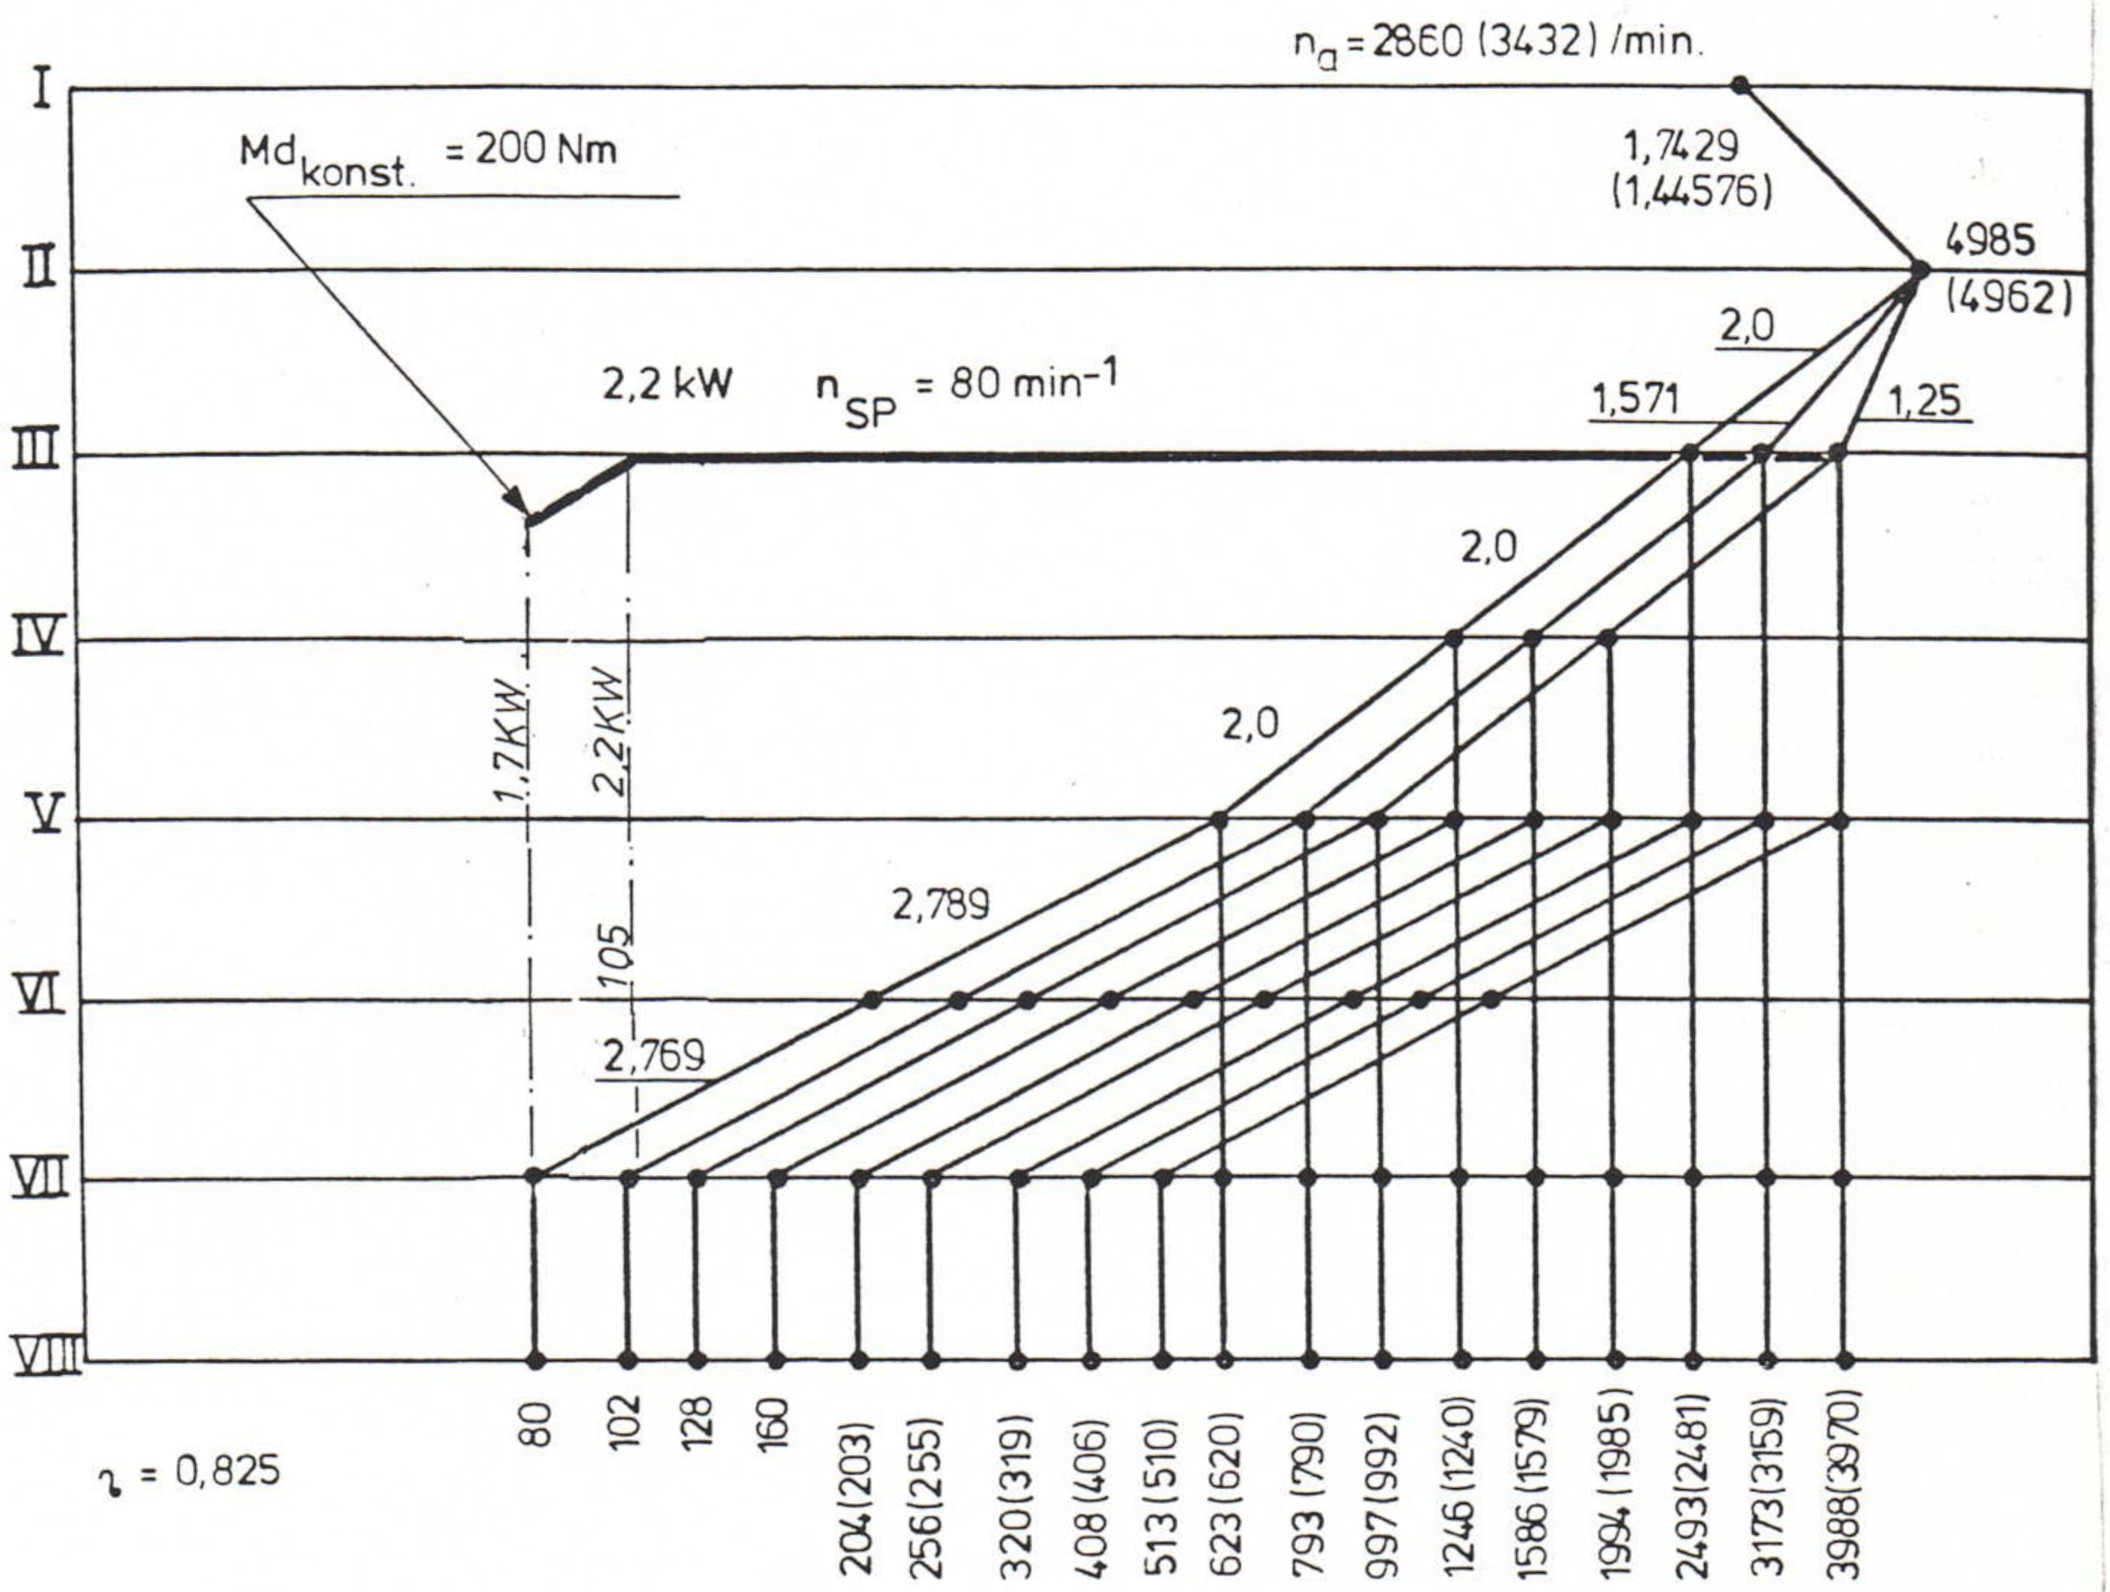
\includegraphics[width=1.05\textwidth]{chapter2/gear_train_speeds.jpg}
\end{figure}

\noindent \rule{1.08\textwidth}{0.5pt}
\footnotesize Standard Speeds: 80,100,125,160,200,250,315,400,500,630,800,1000,1250,1600,2000,2500,3150,4000
\rule{1.08\textwidth}{0.5pt}

\vspace{.5cm}

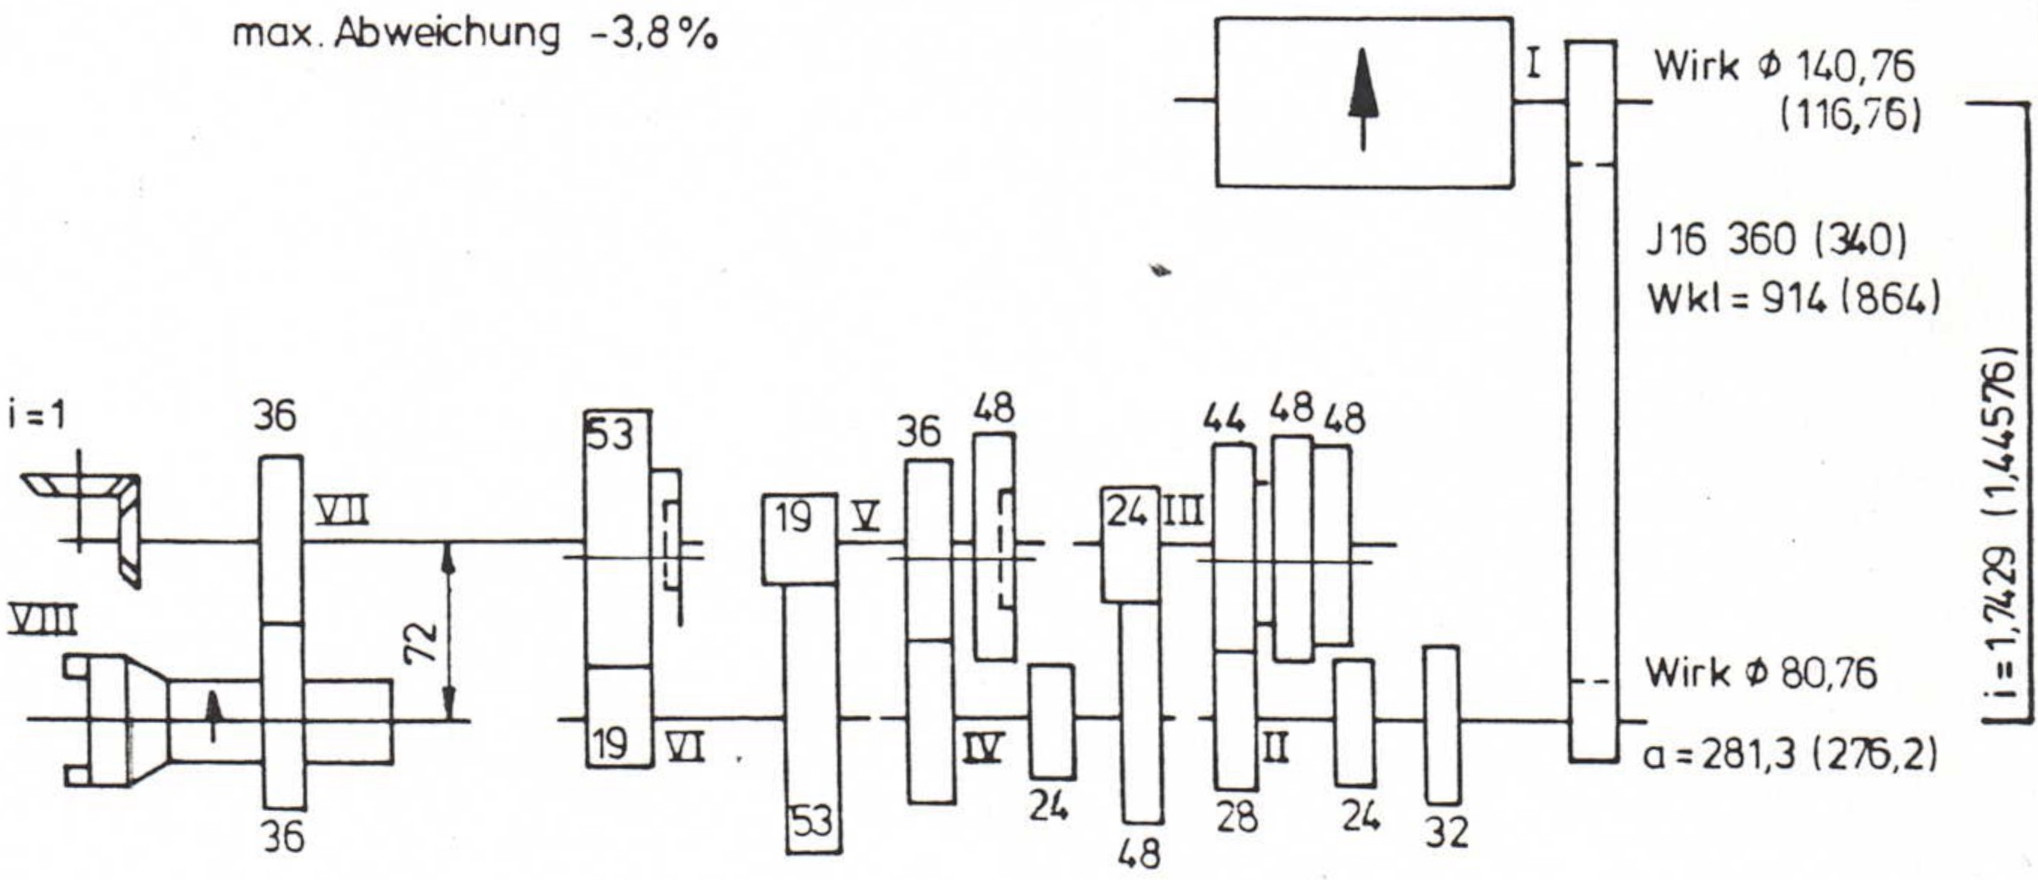
\includegraphics[width=1.02\textwidth]{chapter2/gear_train_layout.jpg}


\end{document}